%% paper04 — 独立小论文稿(中文)
%% 模板: ACM acmart manuscript。正文已与旧 NOSR/HMACSP 叙事脱钩,仅保留版式骨架。
%% 编译: XeLaTeX(必须;见下方 ctex 说明)。
%%
\documentclass[manuscript,screen,review]{acmart}

%% ===================== 中文支持 =====================
%% scheme=plain: 只接管中文字体与断行,不改写 acmart 的章节名。
%% fontset=windows: 本机宋体/黑体; Overleaf/Linux 可改为 fontset=fandol。
\usepackage[UTF8,scheme=plain,fontset=windows]{ctex}

\usepackage{algorithm}
\usepackage{algorithmicx}
\usepackage{algpseudocode}
\usepackage{pifont}
\usepackage{makecell}
\providecommand{\checkmark}{\ding{51}}
%% B13 删去 \cmark/\xmark/\omark:定义后全稿 0 处引用(表格未采用勾叉体例)。原值见 git。
\usepackage{threeparttable}
\usepackage{tikz}
\usetikzlibrary{positioning,arrows.meta,calc,shapes,shadows}
\usepackage{xcolor}
\usepackage{amsmath}
\usepackage{bm}
\DeclareMathOperator*{\argmin}{arg\,min}
\DeclareMathOperator*{\argmax}{arg\,max}
\usepackage{multirow}
\usepackage{enumitem}
\usepackage{booktabs}
\usepackage{graphicx}
\setlength{\headheight}{20.48303pt}

%% scheme=plain 不改浮动体名称,与 paper01 中文稿对齐。
\renewcommand{\figurename}{图}
\renewcommand{\tablename}{表}
\floatname{algorithm}{算法}
\renewcommand{\proofname}{证明}

%% 机制缩写:主语是闭包,不是「修复框架」
\providecommand{\STRC}{\textsc{STRC}}
%% B13 删去 \TBD:全稿 0 处引用,待填项一律用 <待填:...> 明文标记,便于自检抓取。

%% =====================================================================
%% 主结果数字的单一来源。
%%
%% 全部由 STRC/tools/paper_numbers.py 从 STRC/experiments/expanded/*.csv 打印,
%% 数据由 `py -m tools.expand_batch` 生成(默认 5 算例 x 10 种子)。
%% 正文一律用宏,不写字面量;改数只改这里,并同步跑一遍上述两条命令核对。
%%
%% !! 2026-08-16 由 3x5=15 对扩到 5x10=50 对。旧稿所有 /15 结果一律作废。
%%
%% !! 2026-08-16(二次):E2b 由 24/50 变为 50/50。这不是换了算例,而是修掉了
%% !! 一处实现与定义的错配。释放集是一个**预约**集合,而 replay_reroute 原先
%% !! 按**工序**判定是否重路(两段中任一段进闭包就整道重规划)。于是当只有满载
%% !! 段进闭包时,同工序的空载段也被改写,而它的 task 并不在释放集里,遂被记为
%% !! 外侧漂移。26 个失败格上的 84 条漂移预约无一例外都是这种同工序空载段,
%% !! 其中 71 条(85%)在 t_now 之前就已执行完毕——改写它同时违反假设 A2。
%% !! 改为按段判定后漂移归零。据此 prop:outside 的前提 (iii) 才真正被满足,
%% !! 此前的 24/50 测的是实现缺陷,不是边集的物理覆盖度。
%% =====================================================================
\newcommand{\NInst}{5}
\newcommand{\NSeeds}{10}
\newcommand{\NPairs}{50}
%% E1/E3:两项都是满分,写成 \NPairs/\NPairs 以免手抄漏改
\newcommand{\PassMiss}{\NPairs/\NPairs}      % T_impact=0 且种子非空且原解不可行
\newcommand{\FeasRone}{0/\NPairs}            % R1 恢复可行的格数
\newcommand{\FeasRtwo}{\NPairs/\NPairs}      % R2 恢复可行的格数
\newcommand{\PassClosed}{\NPairs/\NPairs}    % E2a 结构闭合(泄漏为 0)
\newcommand{\PassInvar}{\NPairs/\NPairs}     % E2b 外侧字段逐条不变
%% E1 主批次 Cl/|R| 的逐算例极值,出处 tab:e1 表体(0.59/0.57/0.59/0.57/0.56)。
%% 此前该区间在正文三处各写一个值(0.56--0.59 / 0.54--0.57 / 0.54--0.58),即 CONFLICT-3;
%% 现统一由本宏出数。**不要**与下列同值但不同源的量混用:
%%   \ScaleCloHi(0.56) 来自规模扫描 tab:scale 的 k=4 格,是另一批次;
%%   \PubEoneFracLo/Hi 来自外部布局批次,账本独立。
\newcommand{\EoneCloLo}{0.56}
\newcommand{\EoneCloHi}{0.59}
%% 耗时(E3 批次,第 1 级改路、无扩域)
\newcommand{\MsRepairMed}{3.2}
\newcommand{\MsRepairMax}{12.8}
%% 稳定性:E5 上受 A2 约束后两臂改动比例已同区间;主对照改为 E7 的 R2 vs RA。
\newcommand{\ResFracRtwo}{50\%--66\%}
%% E5 批次:R0+ 已走固定前缀解码。降级后道改走同车续路后,18 个预算点越界均为 0。
%% 出处 expanded/e5_cross_curve.csv,`py -m tools.expand_batch --only-e5`。
\newcommand{\RzeroPastLo}{0}
%% ---------------------------------------------------------------------
%% E5 两批合读。pub_batch 直接 import expand_batch 的 _run_e5,
%% t_now_frac=0.35、预算 {0.2,1,2}s、pop=40、hot=True 逐项同一,故可合池;
%% 两批只差布局出处(自建 / 外部转录),这正是合池的意义。
%% 出处 expanded/e5_cross_curve.csv + pub_layouts/e5_cross_curve.csv,
%% 复算脚本 tools/_p17_e5_stats.py。
\newcommand{\EfiveInst}{4}          % congested_8x4x4, example_3x3x2, LyuL2_4m, LyuL6_8m
\newcommand{\EfiveCells}{12}        % 独立算例--随机种子格
\newcommand{\EfivePts}{36}          % 预算点总数 = 12 格 x 3 档
\newcommand{\EfiveWLT}{35/1/0}      % 逐预算点 R0+ 胜/持平/负
\newcommand{\EfiveWinMin}{11}       % 最小预算档上 R0+ 严格更优的格数
\newcommand{\EfiveTieMin}{1}        % 同,持平的格数(LyuL6_8m, 种子 2024)
%% ---------------------------------------------------------------------
%% 离散度口径(P17)。均值表/图一律配一个四分位距,免得只读到均值。
%% 出处同上脚本;E1 为 expanded/e1_miss.csv 逐算例 10 种子。
\newcommand{\EoneFracIqrLo}{0.024}  % 逐算例 Cl/|R| 的 IQR 最小值
\newcommand{\EoneFracIqrHi}{0.049}  % 同,最大值
\newcommand{\EoneFracMed}{0.571}    % 50 对合池中位
%% 合池 IQR 实测 0.0372,与 §5 的 Hodges--Lehmann 估计 0.037 同值\emph{不同源};
%% 为免两个不相干的量在正文里撞成一个结果,此处不出宏、图注也不报该值,
%% 只报逐算例 IQR 区间与合池极差,已足够说明离散度。
\newcommand{\EoneFracMin}{0.500}    % 50 对合池极差下端
\newcommand{\EoneFracMax}{0.655}    % 同,上端
%% phi 扫描(tab:scale / fig:scale):耗时极差与 Cmax 逐档 IQR
\newcommand{\ScaleMsMin}{2.2}       % 全扫描 strc_wall_ms 极差下端
\newcommand{\ScaleMsMax}{23.8}      % 同,上端
\newcommand{\ScaleCmaxIqrLo}{8}     % 逐档 R0+ Cmax 的 IQR 最小值
\newcommand{\ScaleCmaxIqrHi}{76}    % 同,最大值
%% 规模扫描的加速比区间(跨两算例的逐格极值)
\newcommand{\SpeedLo}{87}
\newcommand{\SpeedHi}{3051}
%% E6:A 类上闭包严格大于工序依赖图释放集的格数(其余格两者相等,不是包含失败)
\newcommand{\StrictlyLarger}{87/100}
%% E6:闭包占 t_now 之后活预约的比例(走廊阻断)。这个数偏大,
%% 是「不作最小性主张」那条注记的实测依据,不要美化。
\newcommand{\ClosureAliveFrac}{92\%}
%% =====================================================================
%% 外部来源布局批次(STRC/experiments/pub_layouts/)。**独立账本**,不并入上面的
%% \NPairs 对——把它混进主批次会让全部 /\NPairs 结果改口径。两批算例逐参数同口径,
%% 只差布局来源。数出处:py -m tools.pub_batch 后 py -m tools.paper_numbers。
%% 边权是本文补齐的等权值,故这批数**不可**与 Lyu 或 van Os 的参照值比较。
%% =====================================================================
\newcommand{\NPubInst}{5}
\newcommand{\NPubPairs}{50}
\newcommand{\PubPassMiss}{\NPubPairs/\NPubPairs}
\newcommand{\PubFeasRone}{0/\NPubPairs}
\newcommand{\PubFeasRtwo}{\NPubPairs/\NPubPairs}
\newcommand{\PubPassClosed}{\NPubPairs/\NPubPairs}
\newcommand{\PubPassInvar}{\NPubPairs/\NPubPairs}
\newcommand{\PubEoneFracLo}{0.438}
\newcommand{\PubEoneFracHi}{0.547}
%% E4 同参数对照。**这里的口径要格外小心,曾写错过一次。**
%% \NPubInst 个外部算例只落在 \NPubNets 张不同路网上(4x4 去一条边:LyuL2/L3;
%% 5x5 去两条边:LyuL4/L5/L6),差别在机器台数与落位。于是:
%%   \PubCloSpread 这个极差的两个端点(\PubCloHi=LyuL2 4 机、\PubCloLo=LyuL3 5 机)
%%   **共享同一张路网**,所以它测的是机器落位,**不是**路网几何。
%%   不要再写成"闭包占比随布局显著变化"——数据不支持这句。
%% 正确的用法是:同一路网上换落位即得 \PubCloSpread,而 LU 最小割与漏斗占比全程恒定
%% (两张路网都把装卸站放在网格角点,四邻接下角点恰两条出边),故静态割被干净否证。
%% 注意别把这句写成"公开布局一律放在角点":工具集另附的 Liu 那族放在网格边中点(出度 3),
%% 只是因允许对角移动而未收入。准确的说法是该指标只取到极少数由摆位决定的离散值。
\newcommand{\NPubNets}{2}
\newcommand{\PubCloLo}{0.305}
\newcommand{\PubCloHi}{0.512}
\newcommand{\PubCloSpread}{0.207}
\newcommand{\PubCloSpreadBig}{0.075}
\newcommand{\SelfCloLo}{0.446}
\newcommand{\SelfCloHi}{0.497}
\newcommand{\SelfCloSpread}{0.051}
\newcommand{\PubEfiveNoCross}{17/18}
%% =====================================================================
%% 便宜对照臂(E7)与算例规模扫描(E8)。两批共用同一组臂定义:
%%   RS  全局右移。不改路径/指派/序,把未完成的一切统一后推到阻断窗之后。
%%       冻结判据与 R2 相同(t_end <= t_now 不可动),故按 A2 可采纳。
%%   RD  原染色体重解码。保持机器指派与加工顺序,走与 R0+ 同一套固定前缀解码。
%%       降级后道改走同车续路后,A2 越界为 \RedecodeBad。
%%   RA  不划边界:释放 t_now 之后的全部预约,再走与 R2 完全相同的改路重放。
%%       它与 R2 共用引擎、共用冻结判据,唯一差别是释放集取了平凡上界,
%%       故 R2--RA 之差可全部归因于闭包这个对象本身。
%% 出处:STRC/experiments/cheap_baselines.csv (py -m tools.cheap_baselines)
%%      STRC/experiments/scale_curve.csv     (py -m tools.scale_curve)
%% 协议与 E1--E3 一致(繁忙走廊单窗阻断、t_now=0.35 Cmax、R2 不开扩域),
%% 故 tab:cheap 可与 tab:e3 并读;但**不可**与 tab:e5 并读——那批只有两个算例。
%% =====================================================================
\newcommand{\MsShift}{1.42}          % RS 耗时中位/ms(\NPairs 对)
\newcommand{\MsRedecode}{4.16}       % RD 耗时中位/ms(同上)
\newcommand{\MsAllFuture}{2.76}      % RA 耗时中位/ms(同上)
\newcommand{\MsCheapRtwo}{2.74}      % 同批 R2 的耗时中位,供四臂同口径比较
\newcommand{\RedecodeRatio}{1.5}     % MsRedecode / MsCheapRtwo
\newcommand{\ShiftBad}{0/\NPairs}    % RS 改写已完成预约的格数
\newcommand{\RedecodeBad}{0/\NPairs}
\newcommand{\WinVsShift}{27/16/7}    % R2 对 RS 的 Cmax 赢/平/输
\newcommand{\WinVsRedecode}{14/14/22}
\newcommand{\WinVsAllFuture}{4/46/0}
\newcommand{\ResFracCheapRtwo}{0.540}
\newcommand{\ResFracShift}{0.627}
\newcommand{\ResFracRedecode}{0.618}
\newcommand{\ResFracAllFuture}{0.604}
%% R2 对 RA 的逐格稳定性对比(改动比例;两臂都可行的 \NPairs 格全部纳入)。
\newcommand{\RAStabWTL}{31/18/1}     % R2 更稳/持平/更差
\newcommand{\RAStabP}{8.8\times10^{-7}}  % Wilcoxon 符号秩,双侧
\newcommand{\RAStabMean}{0.064}      % 改动比例平均降幅
%% 下面两个是剔除 6 个「两法恒等」格(R2 释放集 = 全部未结束占用)后的同一结果,
%% 由 STRC/tools/audit_checks.py 自 cheap_baselines.csv 直算;剔除使降幅变大。
\newcommand{\RAStabWTLNet}{31/12/1} % 剔除恒等格后的 R2 更稳/持平/更差(n=44)
\newcommand{\RAStabMeanNet}{0.073}  % 同,平均降幅
\newcommand{\RAStabMed}{0.029}       % 同,中位降幅
\newcommand{\RACmaxRatio}{0.999}     % Cmax 比 R2/RA 均值
\newcommand{\RACmaxLo}{0.970}        % 同,最小值(R2 最占优的那格)
\newcommand{\ClosureShareLo}{0.80}   % 闭包/全部未来预约:最小值
\newcommand{\ClosureShareMean}{0.92} % 同,均值(与 \ClosureAliveFrac 同源)
%% 算例规模梯子:工件 2k、机器 k、车 k,k=4..10;拥堵档、H、F、Tt/Tp 与两处割集同口径,
%% 只有规模变(生成器 clbs/tools/gen_instances.py 的标定见其文档字符串)。
\newcommand{\ScaleKs}{7}
\newcommand{\ScalePairs}{70}
\newcommand{\ScaleJobsHi}{20}
\newcommand{\ScaleMachHi}{10}
\newcommand{\ScaleCloLo}{0.48}       % 闭包占全表比例:k=10
\newcommand{\ScaleCloHi}{0.56}       % 同,k=4
%% 下面三个与上面两个是同一批数据的两种分母,由 tools/audit_checks.py 自 scale_curve.csv
%% 的 n_res / n_live / closure 三列直算(不是反推)。Cl/|R| 的可达上界是 |R^o|/|R|,
%% 故回答「占比会不会涨到接近 1」必须用 Cl/|R^o| 这一口径。
\newcommand{\ScaleAliveShare}{0.61}  % 均 |R^o|/|R|,七档均值 0.611
\newcommand{\ScaleCloAliveLo}{0.78}  % 闭包占尚未结束占用之比,档均值最低:k=10 的 0.782
\newcommand{\ScaleCloAliveHi}{0.91}  % 同,最高:k=4 的 0.905
\newcommand{\ScaleMsHi}{10.4}        % R2 耗时中位:k=10
\newcommand{\ScaleRatioLo}{1.5}      % RD/R2 耗时比:k=4
\newcommand{\ScaleRatioHi}{3.3}      % 同,k=10
\newcommand{\ScaleFeasFirst}{69/\ScalePairs}   % 第 1 级改路即可行的格数
\newcommand{\ScaleFeasAll}{\ScalePairs/\ScalePairs}
%% E7 事后规则:释放占比 vs 稳定性降幅。阈值在 cheap_baselines.csv 本样本上选定,
%% 不作外推定理。出处:py -m tools.paper_numbers(worth_section)/fig_strc_worth_CN.py
\newcommand{\WorthThresh}{0.93}
\newcommand{\WorthLowN}{27}
\newcommand{\WorthLowMean}{0.094}
\newcommand{\WorthHighN}{23}
\newcommand{\WorthHighMean}{0.029}
\newcommand{\WorthVanish}{0.97}
%% 边集差分试探。出处:STRC/experiments/edge_probe.csv (py -m tools.edge_probe --full)
\newcommand{\ProbeLeakPairs}{0/50}
\newcommand{\ProbeLeaks}{0}
%% E6 修复维(第 1 级、不开扩域)。出处:expanded/e6_types.csv 的 R2_feasible 列
\newcommand{\FeasESixBlock}{\NPairs/\NPairs}
\newcommand{\FeasSlow}{\NPairs/\NPairs}
\newcommand{\FeasESixAgv}{\NPairs/\NPairs}
\newcommand{\FeasESixRa}{\NPairs/\NPairs}
%% 非均匀边权 E1/E3。出处:STRC/experiments/weight_sweep.csv (py -m tools.weight_sweep)
\newcommand{\WeightLogRtwo}{\NPairs/\NPairs}
\newcommand{\WeightLuRtwo}{\NPairs/\NPairs}
\newcommand{\WeightSplitRtwo}{49/\NPairs}

\usepackage{amsthm}
\newtheorem{assumption}{假设}
\newtheorem{definition}{定义}
\newtheorem{problem}{问题}
\newtheorem{remark}{注}
\newtheorem{prop}{命题}
\newtheorem{lem}{引理}

\AtBeginDocument{%
  \providecommand\BibTeX{{%
    Bib\TeX}}}

\setcopyright{acmlicensed}
\copyrightyear{2026}
\acmYear{2026}
\acmDOI{XXXXXXX.XXXXXXX}

%%\acmSubmissionID{123-A56-BU3}

\begin{document}

%% =====================================================================
%% 标题:独立小论文用「工序依赖图无法刻画」钩子;大论文章题另用「闭包上的有界修复」
%% B11 定名:题名与正文统一用「工序依赖图」(CONFLICT-4);删「级联」二字——该词全稿
%% 仅题目一处,正文与贡献、结论一律作「失效」,删后逐字一致且全标题回到 29 字(≤30)
%% =====================================================================
\title[工序依赖图无法刻画的走廊占用失效]{时空预约闭包：柔性作业车间中工序依赖图无法刻画的走廊占用失效}

\author{Qi Yu}
\email{230240012@seu.edu.cn}
\orcid{0009-0008-7843-6345}
\affiliation{%
	\department{School of Cyber Science and Engineering}
	\department{Key Laboratory of Computer Network and Information Integration}
	\institution{Southeast University}
	\city{Nanjing}
	\state{Jiangsu}
	\country{PR China}
}

\author{Wei Li}
\orcid{0009-0001-0949-329X}
\email{xchlw@seu.edu.cn}
\authornote{corresponding author}
\affiliation{%
	\department{School of Computer Science and Engineering}
	\department{Key Laboratory of Computer Network and Information Integration}
	\institution{Southeast University}
	\city{Nanjing}
	\state{Jiangsu}
	\country{PR China}
}

\renewcommand{\shortauthors}{Yu and Li}

%% =====================================================================
%% 摘要
%% 骨架:背景缺口 → 主张(边界在预约图) → 对象 STRC → 用法(有界修复) →
%%       与全局重解分工(响应时间一侧) → 实验钩子(不把创新挂在「又一个修复算法」上)
%% =====================================================================
\begin{abstract}
在同时用工序依赖刻画加工先后、又用时间窗预约记录走廊占用的柔性作业车间调度中，
扰动后划定重调度范围的现成做法仍是先找出受影响工序、再连同其后续一并重排。
但走廊在某段时窗内不可通行或通行变慢时，没有任何工序因此无法执行，
该做法给出空范围、判为无需重调度；而落在受扰时段内的走廊占用已经失效，原排程不可行，
等待还会沿让行关系传给后续车辆。缺口不在检测，而在工序依赖图
不含走廊占用之间的让行关系。

本文把重调度范围定义在走廊占用及其依赖关系上，提出时空预约闭包(\STRC)，
其结果集合称为预约影响集：以占用时段与扰动时窗重叠的走廊预约为起点，沿同走廊让行、
同一车辆的后续占用、同一工件与同一机器下一道工序的占用四类边取传递闭包；
集内占用允许改写，集外沿用原计划。依赖边一经给定，一条占用是否属于该集即唯一确定，
不随改路算法的实现而变。恢复分两级：先在集内为原车辆改路，仍不可行时再按既定顺序
扩大允许改写的范围。

实验在 \NInst\ 个算例 \(\times\) \NSeeds\ 个随机种子共 \NPairs\ 对上进行。
走廊阻断时，按工序依赖图划出的范围在 \PassMiss\ 对上均为空，而原排程均已不可行。
改路程序不变、只替换划界对象时，恢复可行率由 \FeasRone\ 变为 \FeasRtwo。
预约影响集对外封闭（集内无指向集外的依赖边）与集外占用的走廊、时段和车辆逐条不变
分别在 \PassClosed\ 与 \PassInvar\ 对上成立。若把允许改写的集合换成
「决策时刻之后尚未结束的全部占用」、其余不变，耗时与完工时间几乎不变，
改动比例则由 \ResFracCheapRtwo\ 升至 \ResFracAllFuture（逐格 \RAStabWTL,
Wilcoxon 符号秩双侧 \(p=\RAStabP\)）。与不改写已结束占用的热启动全局重调度相比，
有界修复耗时低两到三个数量级，但完工时间在全部预算档上均更差，且放宽预算后不出现反超。

主效应来自划界对象的替换：由工序依赖图换为预约影响集后可行性得以恢复，改路程序未变。
次效应来自预约影响集相对「尚未结束的全部占用」的缩减，即改动更少；但前者已覆盖后者的约
\ClosureAliveFrac，两者接近时该收益趋于消失。
集内改路、集外保持与失败后扩大范围沿用既有做法，本文的贡献在于划界对象。
\end{abstract}

\keywords{柔性作业车间调度, AGV 无冲突路由, 时空预约表, 时空预约闭包, 走廊阻断}

%% CCS。投 ACM 时须用官方工具重生成 CCSXML 块;此处先给 \ccsdesc 以消除
%% acmart 对超过两页稿件的 "no CCS concepts" 警告。非 ACM 场合整段可删。
\ccsdesc[500]{Theory of computation~Scheduling algorithms}
\ccsdesc[300]{Applied computing~Industry and manufacturing}
\ccsdesc[300]{Computing methodologies~Planning and scheduling}

\maketitle

%% =====================================================================
\section{引言}
\label{sec:introduction}
%% =====================================================================

\subsection{背景与动机}

考虑运输的柔性作业车间调度长期建立在一个简化假设之上：工件在两台机器之间的移动时间是一个常数，可从按位置对索引的矩阵中读出。
该假设默认车辆互不争用同一路段，行驶时间因此只由两点之间的距离决定，而不是路由决策的结果。
一旦有限车队共享稀疏走廊，并以时间窗预约被争用的路段，行驶时间就不再是固定数据，而成为两个决策的结果：车辆的行驶路径，以及各车辆占用该路段的先后次序。
一辆车的让行会推迟另一辆车的到达，进而推迟后续工序开工及其运输占用。
此时一份可行排程须同时确定工序指派、加工顺序，以及一张记录走廊占用的预约表；扰动既可能使工序无法执行，也可能只使走廊占用失效而不改变任何工序指派。

在开工前一次性完成排程、并把机器指派与无冲突路径一同决定的这类研究已经表明：
当工序可选多台机器时，车辆在走廊上的争用会改变哪台机器更优——通往加工更快的机器的路段若正被占用，加工较慢但更易到达的机器反而更好。
因此，评价候选排程须用时间窗路由计入等待，搜索时还须查询预约表上的冲突，
而不能继续使用常数行驶时间~\cite{vanos2026exact,li2026framework,sun2023integrated}。
上述文献回答的是：在信息完备、尚未开工时，如何排出一份高质量的无冲突排程。同一车间在执行到时刻 \(t_{\mathrm{now}}\) 并发生扰动之后，
问题随之变为：失效落在哪些走廊占用上，改写哪些占用才足以恢复可行，以及能否在不重新启动种群搜索的前提下于毫秒量级内完成恢复。

\subsection{工序依赖图无法刻画的缺口}

%% 措辞收窄(2026-08-16):原句「局部重调度文献常用任务依赖图界定影响域」是一句
%% 针对整支文献的全称否定,一个反例即可推翻——铁路 alternative graph 与 MAPF 都不
%% 在工序依赖图上划界。收窄为「考虑运输的柔性作业车间动态调度这一支」,见 2.5。
在考虑运输的柔性作业车间动态调度研究中，重调度范围通常沿工序依赖图划定。
具体做法是：以因设备故障而无法按原计划执行的工序为起点，把同一工件的后续工序与同一机器上排在其后的工序纳入范围，
或在依赖图上从起点扩展至多 \(\theta\) 步后停止；随后只对范围内的工序重调度。
两篇带 AGV 运输、并以机器故障或插单为扰动的动态调度研究即按此划界——恢复范围分别取「故障后尚未加工的工序」\cite{zhang2023energy}，
与「按扰动影响分为保留、继续、重构三类后的工序与配送任务」\cite{tang2026dynamic}（后者为批量流混合流水车间，扰动含车辆故障，但模型中没有预约表）。
这一做法可上溯至受影响工序重调度（AOR）\cite{zhang2023energy,tang2026dynamic}。
后文以按工序依赖图划界的对照代表这一做法（第~\ref{sec:rw_aor}~节）。

这一划界在扰动本身就是工序事件时往往合理——例如机器故障使若干工序无法按原指派执行。
然而，当排程用时间窗记录走廊占用时，还存在一类扰动：它使某条走廊在某段时间内不可通行，而不改任何工序指派。典型例子是走廊阻断：
走廊在 \([t_a,t_b)\) 时段禁止通行。阻断不修改机器指派或加工顺序，工序依赖图上因此没有任何被直接波及的工序，按该方法划出的重调度范围为空，并据此判为无需重调度。
于是工序依赖图无法刻画这些必须恢复的走廊占用：原计划中与阻断时段重叠的占用已与禁行冲突，不再可行；一辆车因此等待或改道，又会沿让行关系阻塞后续车辆，失效由此在预约表上传播。

这里的「无法刻画」指工序依赖图按定义不含走廊占用之间的让行关系，因而无法表达占用失效在车辆之间的传播。
若运输时间仍取为按位置对索引的常数矩阵，走廊不是可争用的资源，预约表也不存在，这类失效在模型中无从表达；
因此该缺口只存在于用时间窗记录走廊占用的设定中。

据此，本文区分两类扰动。
\begin{itemize}[leftmargin=1.5em,itemsep=0.25em]
\item \textbf{A 类}（作用于工序依赖图）：机械臂故障、加工时间显著偏差、插单，以及\emph{车辆故障}。
这类扰动使部分工序无法按原计划执行，划定重调度范围时的起点工序集非空；
按工序依赖图划界与按预约影响集划界都能给出非空范围，因而不是本文用来检验划界错位的主要对象。
车辆故障归入 A 类的理由见第~\ref{sec:disturbance_classes}~节：它虽不改工序指派，
却使该车承运的工序不可执行，经「车辆到所承运工序」的对应关系，工序依赖图上仍有非空的起点工序集。
\item \textbf{B 类}（只作用于预约表）：走廊阻断、走廊通行变慢，以及局部通行权临时取消等。
这类扰动不使任何工序无法执行，工序依赖图上的起点工序集为空；
与受扰时段重叠的走廊占用非空，以其为起点纳入重调度范围所得的预约影响集也非空。
\end{itemize}
B 类扰动构成对「按工序依赖图划界」这一做法的问题层面反例：模型同时用工序依赖图刻画加工先后、
用时间窗记录走廊占用时，若重调度范围仍只划在工序依赖图上，便无法表达走廊阻断这类扰动。
上引两篇带 AGV 的动态调度研究不考虑车辆之间的走廊争用（第~\ref{sec:rw_position}~节），
工序依赖图是其唯一可用的划界对象；这一错位只在两套对象同时出现时发生（第~\ref{sec:rw_claim}~节）。
图~\ref{fig:motivate} 对照这一缺口：左侧工序依赖图上没有作为起点的工序，因而判为无需重调度；
右侧预约表上，与阻断时段重叠的占用成为起点，并沿让行与接续关系形成预约影响集。

\begin{figure}[t]
\centering
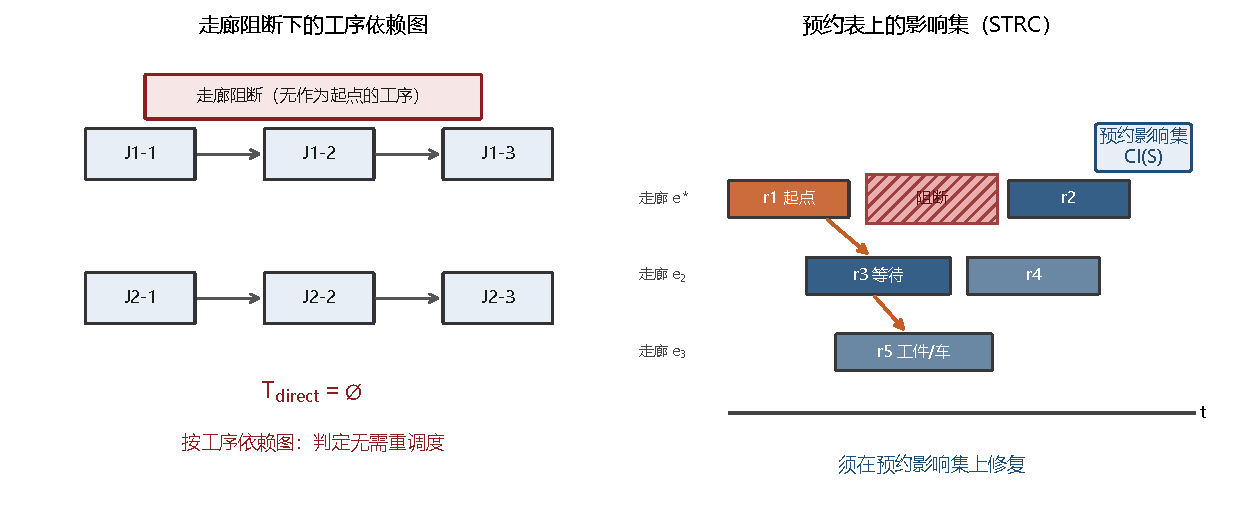
\includegraphics[width=\linewidth]{figures/fig_strc_motivate_CN}
\caption{动机示意。左：走廊阻断不使任何工序或机器无法按原计划执行，工序依赖图上没有作为起点的工序。
右：同一扰动下，与阻断时段重叠的走廊占用成为起点，并沿让行与接续关系形成预约影响集。}
\Description{并排两幅图。左幅是工序依赖图，走廊阻断没有使任何工序节点无法执行，
作为起点的工序集为空。右幅是同一时刻的走廊预约表，与阻断时段重叠的占用成为起点，
这些占用沿让行边与接续边向外连成一片传播区域。}
\label{fig:motivate}
\end{figure}

\subsection{本文主张}

本文有三点主张。

第一，当柔性作业车间用时间窗预约保证车辆无冲突通行时，扰动后的重调度范围应定义在由走廊占用及其让行关系构成的预约依赖图上，而不是只定义在工序依赖图上。

第二，划界方法是时空预约闭包（\STRC, Spatiotemporal Reservation Closure），其结果集合称为预约影响集：
以与扰动时窗重叠、因而失效的走廊占用为起点，沿让行、同一车辆的后续占用、同一工件下一道工序的占用、同一机器上下一道工序的占用，
把直接或间接必须作废、重写的走廊占用全部纳入重调度范围。
这些依赖关系一经给定，影响集以外的占用不再是集内占用沿上述关系的下一步，
因而「改写哪些占用」对应一个可以检验的集合，而不是人为设定的搜索半径。

第三，得到影响集之后，在集内为原车辆改路、集外保持原占用；若仍得不到可行排程，
再按同一工件、同一车辆、直至全部未完成占用的顺序，扩大允许改写的范围。
A 类故障上另允许换车与改派，仍不改加工顺序。
这些步骤沿用既有做法，用于落实影响集并恢复可行排程。

上述三点共用一个立场：\textbf{预约影响集是一次测量，不是一个决策。}
本文不用占用间的让行关系引导搜索以更换指派或路径，因为那属于改进排程决策：
消除一处走廊等待后，另一处约束往往成为新的瓶颈，完工时间上的收益因此容易被抵消。
本文用同一组让行关系划定哪些占用已经失效：依赖关系给定后，
一条占用是否属于影响集，取决于它能否从起点沿这些关系到达，结果唯一确定，
不随之后哪一条约束成为新的瓶颈而改变。

纳入哪些依赖边是建模选择；边集选定后，影响集对外封闭（集内占用没有指向集外的依赖边）
即为定义的推论（命题~\ref{prop:struct}）。
影响集不一定是恢复可行所需的最小占用集合，因为最小集合依赖于允许的修复动作，
而影响集的定义不绑定于任何一种修复方法（注~\ref{rem:minimality}）。

相对以原排程为起点、在限定时间内重新搜索的全局重调度，预约影响集回答的是另一类问题：
在必须很快给出可执行方案时，能否恢复可行，并把改写限制在影响集以内。
在命题~\ref{prop:outside} 的条件下，修复后影响集以外每条走廊占用的走廊、时段与车辆均与原计划一致。
相对不改写决策时刻已经结束的占用的全局重调度，有界修复得到的完工时间 \(C_{\max}\) 更差，
两者的改动比例处于同一量级；有界修复的长处在于算法耗时短得多（毫秒量级对秒量级）。
算法耗时与改动比例须分开解释，第~\ref{sec:cheap}~节对二者分别检验：
耗时短来自对影响集内各段运输各做一次路径规划、不重新启动种群搜索，而不来自影响集本身；
影响集是否减少了改动，无法从上述全局重调度对照中得出（两者比例已经接近），
须另设对照：改路程序相同，唯一差别是允许改写的集合取影响集还是尚未结束的全部占用。
在所测的 \(\EfiveCells\) 个算例--随机种子格上，全局重调度在各搜索时限下得到的 \(C_{\max}\) 均更小。
按工序依赖图划界时，走廊阻断因找不到受影响工序而不会触发局部重调度，原排程保持不可行；
若改为触发全局重调度，则可以恢复可行，但算法耗时为秒级。
因此，本文关注的是须立即恢复可行时走廊占用上失效范围的识别及相应的局部恢复。

\subsection{贡献}
\label{sec:contributions}

本文的贡献如下，后文分别记为 C1、C2、C3。

\begin{enumerate}[label=\textbf{C\arabic*.},leftmargin=2.2em,itemsep=0.4em]
\item \textbf{指出工序依赖图无法刻画的一类失效。}
当排程同时用工序依赖刻画加工先后、又用时间窗记录走廊占用时，
现成的重调度范围仍按受影响工序划定。
走廊阻断、走廊通行变慢等扰动不改任何工序指派，
按该方法划出的范围为空，并据此判为无需重调度；
但与受扰时段重叠的走廊占用已经失效，原排程不可行，
等待还会沿让行关系传给后续车辆。
其根源在于工序依赖图不含占用之间的让行关系。

\item \textbf{把重调度范围定义为预约影响集。}
以与扰动时窗重叠的走廊占用为起点，
沿让行、同一车辆的后续占用、同一工件与同一机器上下一道工序的占用，
把直接或间接必须作废、重写的占用纳入重调度范围；这一划界方法称为时空预约闭包（\STRC）。
依赖关系一经给定，一条占用是否属于影响集唯一确定，
集内占用没有指向集外的依赖边，因而「改写哪些」对应一个可检验的集合，
而不是人为设定的搜索半径，也不随改路算法的实现而变。
\emph{影响集作为划界对象}的证据是：走廊阻断下工序依赖图上的范围为空
而原排程已不可行（\(\PassMiss\)，第~\ref{sec:e1}~节）；预约影响集对外封闭（\(\PassClosed\)，
第~\ref{sec:e2}~节）；A 类扰动下预约影响集包含工序依赖图已纳入的全部占用（第~\ref{sec:e6}~节）；
边界差分试探的泄漏为 \ProbeLeakPairs。
\emph{该划界的净收益}由与 RA 的对照给出（第~\ref{sec:cheap}~节），
即相对「改写全部尚未结束的占用」减少的改动。

\item \textbf{给出与该划界相匹配的局部恢复，并分清各项结果各来自何处。}
在影响集内为原车辆改路、集外保持原占用；仍不可行时再扩大允许改写的范围。
修复步骤沿用既有做法，本项贡献在于通过对照区分各项结果的来源。
在同一套走廊路网、时间窗路由与无冲突校验下对照表明：
按工序依赖图划界时走廊阻断 \(\FeasRone\) 恢复可行，按预约影响集划界时 \(\FeasRtwo\) 恢复可行，
可行与否来自划界对象，而不是改路程序的优劣；
有界修复以毫秒级耗时恢复可行，但完工时间 \(C_{\max}\) 较全局重调度更差，
且放宽预算不出现反超（\(\EfiveCells\) 个算例--随机种子格，所测预算区间内无交叉点）；
与「改写全部尚未结束的占用」的对照相比，耗时与 \(C_{\max}\) 几乎不变，
只有改动的减少可归因于影响集（第~\ref{sec:cheap}~节）。
在四类扰动与两种划界的交叉中，工序依赖图上的范围仅在走廊阻断与通行变慢下为空，
预约影响集均非空，且在机械臂故障与车辆故障下包含工序依赖图上的范围。
\end{enumerate}

同一车间、同一预约表上，开工前的一体化排程用预约表构建无冲突方案~\cite{vanos2026exact,li2026framework,sun2023integrated}；本文在执行时刻用预约表定位失效范围，二者作用于不同阶段。

\subsection{篇章结构}

第~\ref{sec:related_work}~章按四类回顾相关工作：作业车间如何按工序或时间轴划定重调度范围、
铁路调度如何表达排他资源上的占用先后、无冲突多车路径如何做局部重规划，
以及考虑运输的柔性作业车间把边界划在何处，并据此说明本文的位置。
第~\ref{sec:problem}~章给出走廊预约设定与执行期恢复问题：
车间、走廊预约表与工序依赖图，两类扰动，以及恢复须满足的条件。
第~\ref{sec:strc}~章定义时空预约闭包及其结果集合预约影响集，说明其依赖边与对外封闭等性质
（图~\ref{fig:graphs}、\ref{fig:closure}）。
第~\ref{sec:repair}~章说明如何在影响集内为原车辆改路、集外保持原占用，
以及仍不可行时如何扩大允许改写的范围，并与全局重调度对照（图~\ref{fig:framework}）。
第~\ref{sec:experiments}~章报告可行性、算法耗时、占用改动比例与完工时间，
并用案例甘特图在工序时间轴上展示统计结果对应的改动形态。
第~\ref{sec:conclusion}~章总结全文，并讨论局限与后续工作。

%% =====================================================================
\section{相关工作}
\label{sec:related_work}
%% =====================================================================

%% 相关工作按问题类型回顾,不作「四层定位」。旧文献以引文簇保留,叙述以近作为主。

动态调度的一个基本问题是：扰动发生后，重调度范围划在什么对象上，即改哪些、其余保持不动。
已有文献把这一范围划在不同对象上——工序或时间轴、排他资源上的占用先后、
受影响的车辆，以及带运输的柔性作业车间中的工序集合。
下面按这四类回顾各自做了什么、尚未覆盖什么，并在表~\ref{tab:position} 中做汇总。

\subsection{作业车间的局部重调度}
\label{sec:rw_aor}

对机器故障、插单等工序事件，按受影响工序划定重调度范围，在带 AGV 的动态调度中仍被采用。
Zhang 等~\cite{zhang2023energy} 处理机器故障与插单，恢复范围取故障后尚未加工的工序；
Tang 等~\cite{tang2026dynamic} 按扰动影响把工序与配送任务分为保留、继续、重构，
并把完全重调度、部分重调度与右移并列，指出右移保住稳定性、让出优化空间。
本节与下节据以定位的转述，所本原句一并列于表~\ref{tab:refcheck}。
这一做法可上溯至受影响工序重调度(AOR)~\cite{abumaizar1997rescheduling,subramaniam2003maor}：
只重排被扰动直接或间接波及的工序。
沿时间轴划界与失败后扩大范围同样已有文献研究过，包括 match-up~\cite{akturk1999matchup}
与增量扩大时间窗的 Local Rescheduling~\cite{kuster2007local}。
右移则不判定谁受影响，把未完成部分整体后推。
滚动时域与分解式方法在规模与质量之间折中~\cite{zeitrag2025novel,zhao2019decomposition}；
综述见~\cite{vieira2003rescheduling,ouelhadj2009survey}。

这些工作表明，划定范围再局部重调度并不是新问题，前提是扰动首先作用在工序上。
一旦扰动只使走廊不可通行而不改指派，按该方法划出的范围可以为空，原排程却已不可行。

\subsection{排他资源上的占用先后}
\label{sec:rw_ag}

「谁先占用同一排他资源」被建成图，在铁路调度中已有系统研究。
Mascis 与 Pacciarelli~\cite{mascis2002alternative} 的 alternative graph
把析取图推广为：顶点是作业对闭塞区段的占用，固定弧表示路径先后，
成对的 alternative arc 表示谁先通过该区段。
D'Ariano 等人~\cite{dariano2007branch} 用该模型做列车实时重调度，
扰动后重算无冲突时刻表，并尽量接近原计划。
同走廊上的让行关系与 alternative arc 表达的是同一类先后。

与本文不同的是用法。对每一处争用，alternative graph 给出两条互斥的弧
（甲先通过，或乙先通过），排程就是从中选定一条：
选定后图中不能出现正权回路，时刻表才可行，并尽量使目标最优——占用先后因此是决策变量。
本文的计划已经排好，谁先通过哪条走廊已经确定，不再选择先后，
只按这些既定的让行与接续关系，把扰动后必须作废的原走廊占用纳入重调度范围。
此外，铁路模型把闭塞区段当作机器，工序与占用在同一张图上，
区段不可用即为工序事件，因此不存在「范围划在工序依赖图上而遗漏走廊阻断」的问题。
柔性作业车间中加工与走廊占用是两套对象，现有的 AOR 划界并不利用占用先后关系。

\subsection{无冲突多车路径的局部重规划}
\label{sec:rw_mapf}

在多智能体路径规划中，只为受影响者进行重调度、其余视为动态障碍，已是标准做法。
Švancara 等人~\cite{svancara2019online} 在在线 MAPF 中给出
% selfcheck:allow-term 「受影响集合」此处指 MAPF 独立性检测的输出,不是本文机制的名字
Replan All、Replan Single 与 Replan Affected，并用在线独立性检测确定受影响集合；
Malka 等人~\cite{malka2024online} 在地图不准确时，同样只为受观测变化影响的车辆重规划。
% selfcheck:allow-term 「时空占用」是 MAPF 的既有术语,此处在转述该文献,不指本文的走廊占用
无冲突路径规划把时空占用作为一等约束，但起终点通常由外部给定~\cite{zhang2024guidance}。

上述做法已经把「只改受影响者、其余保持原计划」做成标准机制，本文沿用这一机制。
与本文设定的不同在于：这类工作只有车辆的起终点，没有工件—工序—机器指派，
因而不会出现「重调度范围按工序依赖图划定、走廊阻断因找不到受影响工序而被遗漏」的情形。
% selfcheck:allow-term 「受影响集合」此处是两法共用的中性说法,后半句即在说它是检测算法的输出
就受影响集合如何得到而言，MAPF 用独立性检测找出受影响车辆，得到的是检测算法的输出，随实现方式和停止条件而变。
本文给出的预约影响集则不同：依赖边一经给定，一条占用是否属于该集，
只取决于它能否从起点沿这些边到达，与随后用哪一种改路算法无关
（第~\ref{sec:containment}~节）。

\subsection{考虑运输的柔性作业车间调度}
\label{sec:rw_position}

考虑运输车辆的柔性作业车间调度已有系统综述~\cite{xin2025review}。
近期组合优化工作仍普遍把行驶时间取为按位置对索引的常数矩阵，
并在此之上发展约束规划、元启发式与知识引导搜索~\cite{meng2025cp,qin2026knowledge,fu2025integrated}。
该约定下车辆并不争用同一路段，走廊阻断在模型里没有对应对象，无法被检验。

一旦用时间窗记录走廊占用，加工先后与走廊占用同时进入模型。
拥堵感知派车可用局部密度等代理量选车，而不改机器指派~\cite{kim2026congestion}。
把柔性指派与无冲突运输联合建模的工作相对较少：
van Os 与 Basten~\cite{vanos2026exact} 形式化了带无冲突运输约束的柔性作业车间调度，
并以分解方法在多数基准算例上取得可证最优，少数因限时未能保证最优性；
两阶段方案先固定排产再消解车辆冲突~\cite{sun2023integrated}；
亦有学习层排产、路径层消冲突、并以有限反馈连接的框架~\cite{li2026framework}。
但这些工作回答的是开工前如何排出可行且质量好的无冲突排程。

在本节所引工作中，走廊预约表与执行期扰动响应未同时出现：含预约表的工作排除了执行期故障，
处理执行期扰动的工作则没有预约表。
例如（原句见表~\ref{tab:refcheck}）：
Zhang 等~\cite{zhang2023energy} 在建模假设中写明忽略 AGV 之间的碰撞；
Sun 等~\cite{sun2023integrated}
用时间窗 Dijkstra 消解车辆冲突，却在假设中写明不考虑车辆的充电与故障、车辆始终可用，
并把设备维护与故障列为后续研究。

因此，缺口来自两个条件未同时具备：
工序级划界之所以成立，往往因为模型中没有走廊预约；含预约表的设定又排除了执行期扰动。
两者同时出现时，可直接沿用的只有按受影响工序划界的做法，
而它对不改变工序指派的走廊阻断给出空范围（第~\ref{sec:e1}~节实测 \PassMiss）。
本文处理的正是这一情形。

\begin{table}[t]
\centering
\caption{本文据以划出缺口的五处转述及被引原文（照录英文原句）。}
\label{tab:refcheck}
\footnotesize
\begin{tabular}{@{}p{0.23\linewidth}p{0.55\linewidth}p{0.14\linewidth}@{}}
\toprule
\textbf{本文的转述} & \textbf{被引原文} & \textbf{原文位置} \\
\midrule
Zhang 等~\cite{zhang2023energy} 的恢复范围取故障后尚未加工的工序 &
\emph{``Rearrange the unprocessed operations of current scheme considering the limit of
machine breakdown''} &
重调度流程 \\
\addlinespace
Zhang 等~\cite{zhang2023energy} 在建模假设中写明忽略 AGV 之间的碰撞 &
\emph{``The collision of AGVs are ignored.''} &
建模假设第 (7) 条 \\
\addlinespace
Tang 等~\cite{tang2026dynamic} 按扰动影响把工序与配送任务分为保留、继续、重构 &
\emph{``an event-driven partial rescheduling strategy is proposed, in which the disrupted
operations and delivery tasks are classified into three categories: retained, continued,
and reconstructed''} &
摘要 \\
\addlinespace
van Os 与 Basten~\cite{vanos2026exact} 在多数基准算例上取得可证最优，
少数因限时未能保证最优性 &
\emph{``For most benchmark instances, our LBBD-based approach finds optimal makespan
values. Because of time boxing, only in a few cases, the optimality of the found solution
cannot be guaranteed.''} &
摘要 \\
\addlinespace
Sun 等~\cite{sun2023integrated} 假定车辆始终可用、不考虑故障与充电，
并把设备维护与故障列为后续研究 &
\emph{``It does not consider the charging problem and fault problem of the AGVs, and AGVs
are always available''}；\emph{``Breakdowns and charging problems are not taken into
account.''}；\emph{``Future research will investigate the impact of equipment maintenance
and breakdowns on production scheduling''} &
假设列表、后续工作 \\
\bottomrule
\end{tabular}
\end{table}

\subsection{本文定位}
\label{sec:rw_claim}

\begin{table*}[t]
\centering
\caption{相关工作按\emph{划界对象}分类：每类工作把扰动后「需要改写什么」定义在哪种对象上。
「边界划在」为重调度范围所依附的对象；「有工序依赖图?」兼答该图是否与占用同图；
末行加粗者为本文所处的类别。}
\label{tab:position}
\small
\begin{tabular}{@{}p{0.16\linewidth}p{0.22\linewidth}p{0.14\linewidth}p{0.14\linewidth}p{0.24\linewidth}@{}}
\toprule
\textbf{类别} & \textbf{代表工作} & \textbf{边界划在} & \textbf{有工序依赖图?} & \textbf{与本文的关系} \\
\midrule
作业车间局部重调度 &
AOR~\cite{abumaizar1997rescheduling,subramaniam2003maor};
match-up~\cite{akturk1999matchup};
LRS~\cite{kuster2007local}；
带 AGV 的动态调度~\cite{zhang2023energy,tang2026dynamic} &
工序 / 时间窗 & 有 &
后文对照复现按工序划界与右移 \\
\addlinespace[2pt]
排他资源占用先后 &
alternative graph~\cite{mascis2002alternative}；
铁路实时重调度~\cite{dariano2007branch} &
闭塞区段占用 & 有，与占用在同一张图 &
让行关系同类；铁路用它选择车辆的先后，本文用既定先后划定需要改写的占用 \\
\addlinespace[2pt]
无冲突多车路径 &
Online MAPF~\cite{svancara2019online,malka2024online};
LMAPF~\cite{zhang2024guidance} &
受影响车辆 & 无 &
集内改路、集外保持已是标准做法 \\
\addlinespace[2pt]
带运输的柔性作业车间 &
常数矩阵~\cite{xin2025review,meng2025cp,qin2026knowledge,fu2025integrated}；
一体化排程~\cite{vanos2026exact,sun2023integrated,li2026framework} &
工序集合 & 有；预约表与执行期扰动未同时出现 &
\textbf{本文的位置} \\
\bottomrule
\end{tabular}
\end{table*}

综上，在考虑 AGV 无冲突路由的柔性作业车间中，排程同时用工序依赖刻画加工先后，
又用时间窗记录走廊占用。此时会出现前节所指缺口对应的情形：
走廊阻断等扰动并不使工序无法执行，原指派仍然有效，
但与受扰时段重叠的走廊占用已经失效，原排程不可行。
后文按工序依赖图划界的对照，复现的是第~\ref{sec:rw_aor}~节的做法。
本文主张把重调度范围改到走廊占用及其让行、接续关系上，得到由这些关系唯一确定的预约影响集。

%% =====================================================================
\section{走廊预约设定与执行期恢复问题}
\label{sec:problem}
%% =====================================================================

\subsection{系统设定与记号}
\label{sec:system_brief}

问题设定沿用带无冲突运输约束的柔性作业车间~\cite{vanos2026exact}。
本节一次写清后文用到的对象。一份可行排程 \(\mathcal{S}^0\) 视为给定输入：
它在 \(t=0\) 如何被搜索出来，不影响后文如何划定须改写的占用。

\subsubsection{车间与四组决策}
\label{sec:shop}

车间路由图 \(G=(V,E)\) 强连通。每台机器 \(m\) 由位于固定节点 \(\mathrm{loc}(m)\) 的机械臂执行加工，
下文的机械臂故障即指该机器失效；
\(v_0\in V\) 为装卸站。\(n\) 个工件、机器集合 \(M\)、同构单载车队
\(K=\{1,\ldots,N_A\}\)。工件 \(j\) 有固定工序链 \(O_{j1}\to\cdots\to O_{jn_j}\)；
工序 \(O_{ji}\) 的候选机器集为 \(\Omega_{ji}\subseteq M\)，在机器 \(m\) 上耗时
\(t^P_{jim}\)。一份完整排程同时确定四组决策：
(i)~每道工序的机器指派 \(x\);
(ii)~各机器上的工序加工顺序 \(\pi\);
(iii)~各次搬运的车辆指派 \(y\);
(iv)~每次车辆移动在 \(G\) 上的无冲突路径。
记
\[
\mathcal{S}=(x,\,\pi,\,y,\,R),
\]
其中预约表 \(R\) 是第 (iv) 组的显式记录，定义见下。

运输任务由指派\emph{派生}，不是输入：仅当相邻两道工序不在同一节点时才产生一次搬运。
一次搬运拆成两段——空载取货与满载送达——各段有自己的任务标签 \(u\)
（例如 \(O_{ji}\) 的空载段与满载段是两条记录）。装卸时间取为零：满载段在空载段抵达与工件就绪
二者中较晚的时刻起行，而送达时刻同时就是机器可开工、车辆可接新任务的时刻。
后文允许改写哪些占用、哪些占用保持原计划，以及如何改路，都以段为粒度，而不是整道工序。

\subsubsection{走廊预约与无冲突}
\label{sec:reservation}

每条走廊 \(e\in E\) 是排他资源，通行时间 \(\tau_e\) 已知；两个方向共享同一份占用，
因而任一时刻至多一辆车占用 \(e\)，迎面冲突与同向超车一并排除。
占用取半开区间：第二辆车可以恰好在区间右端点进入。
节点上设容量充裕的停靠位，等待发生在节点上且总是被允许。
一条预约记录为
\[
r=(e,\,[t^s,t^e),\,k,\,u)\in R,
\]
即车辆 \(k\) 在 \([t^s,t^e)\) 占用走廊 \(e\)，所属运输段为 \(u\)。
同一走廊上任意两次不同占用必须满足
\([t^s,t^e)\cap[t^{s\prime},t^{e\prime})=\varnothing\)。
路径只写入 \(R\) 报告为空闲的时窗，故无冲突由构造保证。

时间窗路由是后文改路与各对照方法共用的原语：给定起终点、最早出发时刻与当前 \(R\)，
它返回一条与已有占用无交的通路及各走廊进入时刻。
实现上采用时间窗 Dijkstra~\cite{sun2023integrated}；本文不改这条原语，
只改\emph{哪些}运输段被送进路由器。
与 van Os 预约节点、Lyu 另加节点容量不同~\cite{vanos2026exact,lyu2019approach}，
本文预约的是边；第~\ref{sec:limitations}~节交代由此带来的算例口径限制。

\subsubsection{工序依赖图与预约依赖图}
\label{sec:two_graphs}

% selfcheck:allow-term 「任务图」是 B13 裁定保留的同义登记,兼作 \(G_T\) 下标的来由
工序依赖图 \(G_T=(T_T,E_T)\)（文献中亦称任务图，下标 \(T\) 取自 task）以工序为顶点，
边为工件先后与同机先后；
它\emph{不含}走廊占用之间的让行关系。
预约依赖图 \(G_R=(R,E_R)\) 以 \(R\) 中的占用为顶点，边为让行、同车、同工件与同机所诱导的依赖
（定义~\ref{def:dep}）。
两张图的顶点集不相交：一边是加工，一边是通行。
因此存在一类只改走廊时窗、不改任何工序参数的扰动——按 \(G_T\) 划界时找不到作为起点的工序，
而按 \(G_R\) 划界时起点占用非空，且原排程已不可行。
图~\ref{fig:graphs} 对照这两张图；图~\ref{fig:motivate} 给出走廊阻断下的后果；
表~\ref{tab:notation} 汇总本节及后文用到的记号。

\begin{figure}[t]
\centering
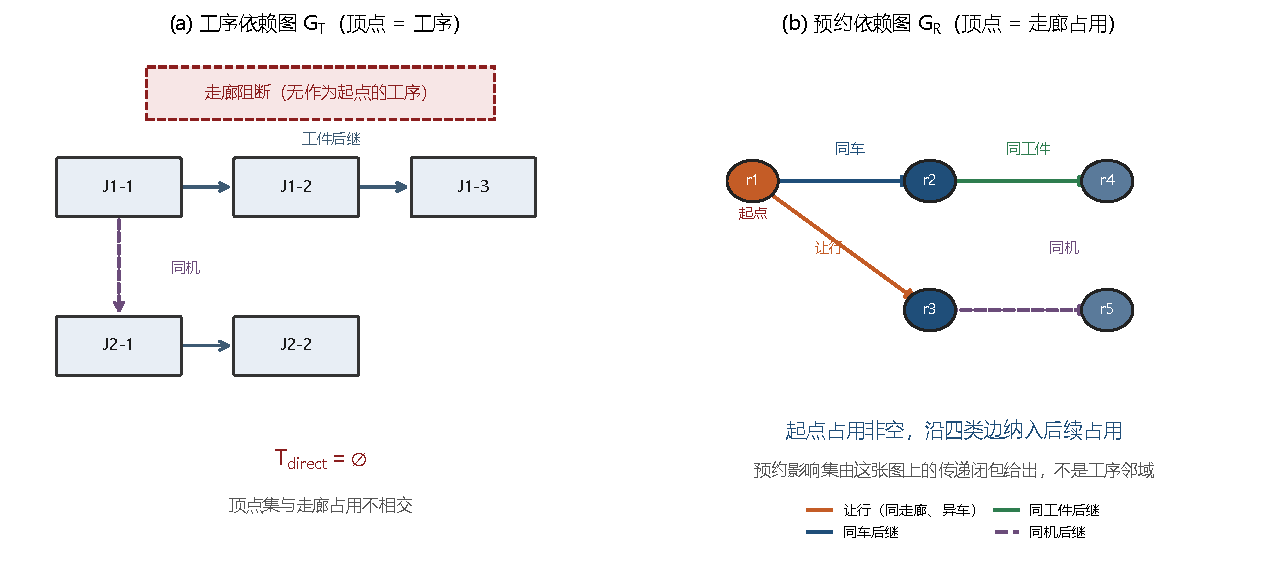
\includegraphics[width=\linewidth]{figures/fig_strc_graphs_CN}
\caption{两张图的顶点集不相交（构造示意）。
(a)~工序依赖图 \(G_T\)，顶点是工序，走廊阻断找不到作为起点的工序；
(b)~预约依赖图 \(G_R\)，顶点是走廊占用，从与阻断窗重叠的占用出发，沿四类依赖边
（让行、同车、同工件、同机；定义~\ref{def:dep}）纳入后续占用。}
\Description{并排两幅。左幅是工序依赖图，工件后继与同机后继连在工序方框之间，
顶部一条虚线框标出走廊阻断，阻断没有落在任何方框上。
右幅是预约依赖图，五个圆形顶点表示走廊占用，四条不同颜色的箭头分别标为
让行、同车、同工件与同机。}
\label{fig:graphs}
\end{figure}

\begin{table}[t]
\centering
\caption{本文常用记号}
\label{tab:notation}
\small
\begin{tabular}{@{}ll@{}}
\toprule
\textbf{符号} & \textbf{含义} \\
\midrule
\(G=(V,E)\), \(\tau_e\) & 走廊路网；走廊 \(e\) 的通行时间 \\
\(v_0\), \(\mathrm{loc}(m)\) & 装卸站；机械臂 \(m\) 所在节点 \\
\(x,\pi,y\) & 机器指派、加工顺序、车辆指派 \\
\(R\), \(r=(e,[t^s,t^e),k,u)\) & 预约表；一条半开占用（车辆 \(k\)，段标签 \(u\)）\\
\(G_T\) / \(G_R\) & 工序依赖图 / 预约依赖图 \\
\(\mathcal{S}^0,\mathcal{S}'\) & 扰动前排程、恢复后排程 \\
\(\mathcal{D},\,t_{\mathrm{now}}\) & 扰动事件、发生（决策）时刻 \\
\(T_{\mathrm{direct}},\,T_{\mathrm{impact}}\) & 工序依赖图上直接受扰的工序 / \(\theta\)-步纳入范围 \\
\(\mathrm{Src}(\mathcal{D})\), \(U\) & 作为起点的占用；允许改写的占用集合 \\
\(\mathrm{Cl}(\cdot)\) & 预约影响集（由 \STRC 得到）\\
\(\varphi\) & 受扰未来工序比例（规模扫描）\\
\bottomrule
\end{tabular}
\end{table}

\subsection{执行期假设}
\label{sec:assumptions}

执行期约定与物理设定如下。其中 A1--A4 由全部对照方法共用，以便把结果归因到重调度范围
如何划定，而不是模型差异；A5 只约束本文方法，全局重调度对照的允许动作更宽（见该条末句）：

\begin{enumerate}[label=\textbf{A\arabic*.},leftmargin=*,topsep=2pt,itemsep=2pt]
\item \textbf{初始排程可行。} \(\mathcal{S}^0\) 在扰动前通过无冲突校验；预约表与工序时间表一致。
\item \textbf{已完成占用不回溯。} 只改写 \(t^e>t_{\mathrm{now}}\) 的尚未结束占用
与未完工工序；\(t^e\le t_{\mathrm{now}}\) 的占用字段不可改写。
\item \textbf{单次、完全观测。} 扰动在 \(t_{\mathrm{now}}\) 被完整观测，且不与其它扰动叠加；
扰动流、预测误差与滚动响应不在本文范围内。
\item \textbf{走廊排他、缓冲充裕、车队同构单载。} 走廊仍为排他半开资源，阻断以附加占用
（或禁行窗）注入路由层。有限缓冲、充电、加减速与装卸时长不建模；
全部车辆在计划开始时空载停于 \(v_0\)。
\item \textbf{允许的恢复动作。} B 类扰动保持原机器指派 \(x\) 与加工顺序 \(\pi\)，只改路；
失败时扩大允许改写的占用集合。A 类故障额外允许：车辆故障把故障车从车队摘除并换车；
机械臂故障把未完工工序改派到其它可行机。加工顺序 \(\pi\) 始终不变，不重开搜索。
实验中的全局重调度对照可以改 \(x\) 与 \(\pi\)（第~\ref{sec:vs_r0}~节）。
\end{enumerate}

\subsection{扰动二分}
\label{sec:disturbance_classes}

\begin{definition}[A/B 类扰动]
\label{def:ab}
若扰动直接使某些工序的指派或\emph{可执行性}失效（机械臂故障、显著工时偏差、插单、
车辆故障等），称其为 \textbf{A 类}；若扰动只使某些走廊时窗不可用、而不使任何工序
不可执行（走廊阻断、走廊通行变慢等），称其为 \textbf{B 类}。
\end{definition}

\begin{remark}[车辆故障为何属于 A 类]
\label{rem:agv_class}
车辆故障不改动任何工序的机器指派，乍看应与走廊阻断同类。但定义~\ref{def:ab} 的判据是
\emph{可执行性}而非指派：车辆发生故障后，它承运的工序在原计划下无法开工，
故经「车辆\(\to\)所承运工序」的映射，工序依赖图上仍有作为起点的工序。这一归类把车辆故障
划到按工序划界能够给出非空范围的一侧。
只有当重调度方法维护了车--任务映射时，这些起点工序才非空；若方法只跟踪工序与机器
（AOR 的常见实现即如此），车辆故障同样会得到空范围。
第~\ref{sec:e6}~节按维护了该映射的口径报告 A 类结果。
\end{remark}

\begin{definition}[工序依赖图上的直接集与影响域]
\label{def:task_impact}
对扰动 \(\mathcal{D}\)，令 \(T_{\mathrm{direct}}(\mathcal{D})\) 为因机械臂故障、车辆故障或工序失效
而无法按原计划执行的工序集合。对 B 类走廊扰动约定 \(T_{\mathrm{direct}}=\varnothing\)。
在 \(G_T\) 上从 \(T_{\mathrm{direct}}\) 出发，按工件后继与同机后继纳入深度至多 \(\theta\) 的工序，
记为 \(T_{\mathrm{impact}}(\mathcal{D},\theta)\)。
\end{definition}

\begin{definition}[作为起点的占用]
\label{def:seeds}
起点集 \(\mathrm{Src}(\mathcal{D})\subseteq R\) 按扰动类型给出，一律只取
\(r.t^e>t_{\mathrm{now}}\) 的占用。
\begin{enumerate}[label=(\alph*),leftmargin=1.6em,itemsep=0.15em]
\item \textbf{走廊阻断/降速} \(\mathcal{D}=(e,[t_a,t_b))\):
\(\{\,r:\ r.e=e,\ [r.t^s,r.t^e)\cap[t_a,t_b)\neq\varnothing\,\}\)。
多处短暂阻断时取各窗起点占用之并。两者共用这条起点规则（原排程按时长未缩放的 \(\tau\) 写出，
与窗重叠的占用都已失效），故划定须改写的占用时二者给出同一个预约影响集——第~\ref{sec:e6}~节据此说明
为何不把二者的划界结果算作两次独立验证；改路时二者处理不同：阻断写为禁行窗，
降速只按倍率缩放与窗重叠部分的通行进度。
\item \textbf{车辆故障} \(\mathcal{D}=(k)\)：该车在 \(t_{\mathrm{now}}\) 之后的全部占用
\(\{\,r:\ r.k=k\,\}\)。
\item \textbf{机械臂故障} \(\mathcal{D}=(m,F)\),\(F\) 为该机上尚未完工的工序：
对每个工件取 \(F\) 中最小工序号 \(i_{\min}(j)\)，起点占用为各工件自该工序起（含）的全部
尚未结束占用。之所以沿工件链向后取而不只取该工序自身，是因为进站运输可能已在
\(t_{\mathrm{now}}\) 前结束，若只取自身，预约影响集会短于工序依赖图上的影响域，对照即不公平。
\end{enumerate}
\end{definition}

\begin{prop}[B 类上工序依赖图给出空范围]
\label{prop:miss}
设 \(\mathcal{D}\) 为走廊阻断。若采用定义~\ref{def:task_impact} 对 B 类的约定，则
\(T_{\mathrm{direct}}(\mathcal{D})=\varnothing\)，从而对任意有限 \(\theta\ge 0\) 有
\(T_{\mathrm{impact}}(\mathcal{D},\theta)=\varnothing\)。
若此外 \(\mathrm{Src}(\mathcal{D})\neq\varnothing\)，则 \(\mathcal{S}^0\) 在 \(\mathcal{D}\) 下不可行。
\end{prop}

\begin{proof}
走廊阻断只使走廊时窗不可用而不使任何工序不可执行，故按定义~\ref{def:ab} 属 B 类。
这一步用到两条前提：阻断窗 \([t_a,t_b)\) 有限，且由假设 A4 缓冲充裕，车辆可在窗外通行；
因而即使阻断期内路网被割断，也没有工序变得不可执行，只是被推迟。若阻断无限期、
或缓冲不足以支持等待，该扰动按定义~\ref{def:ab} 就该归 A 类，不在本命题范围内。
既属 B 类，
再由定义~\ref{def:task_impact} 对 B 类的约定，\(T_{\mathrm{direct}}=\varnothing\)。
\(\theta\)-步纳入的起点为空，故 \(T_{\mathrm{impact}}=\varnothing\)。
若存在 \(r\in\mathrm{Src}(\mathcal{D})\)，则 \(r\) 的占用区间与禁行窗相交。
将 \(\mathcal{D}\) 解释为该走廊上的强制占用后，\(r\) 与禁行窗在同一排他资源上时间重叠，
违背半开时窗无冲突条件（假设 A4 的走廊排他），故 \(\mathcal{S}^0\) 不可行。
\end{proof}

命题~\ref{prop:miss} 是问题层面上的反例。前半句由定义~\ref{def:task_impact} 对 B 类的约定直接得到
（工序依赖图按定义不含走廊占用之间的让行关系，因而无法刻画走廊阻断）；
非平凡的是后半句——起点占用非空时原排程已经不可行，
因而「工序依赖图上范围为空 \(\Rightarrow\) 无需重调度」在用时间窗预约走廊的设定下不成立。
该反例不依赖任何修复算法；实验第~\ref{sec:experiments}~节给出算例规模。

\subsection{恢复问题}
\label{sec:recovery_problem}

\begin{problem}[按预约表划定范围的有界修复]
\label{prob:recovery}
给定可行排程 \(\mathcal{S}^0\)、扰动 \(\mathcal{D}\) 与时刻 \(t_{\mathrm{now}}\)，
求 \(\mathcal{S}'\)，使得：
(i)~\(\mathcal{S}'\) 在 \(\mathcal{D}\) 下通过无冲突校验；
(ii)~未纳入改写范围的占用，其走廊、时段与车辆尽可能与 \(\mathcal{S}^0\) 一致；
(iii)~算法耗时受预算约束。
次级目标为完工时间 \(C_{\max}(\mathcal{S}')\)。
\end{problem}

求解拆为两步：先划定允许改写的占用集合 \(U\subseteq R\)；
再只对 \(U\) 内运输改路，集外占用保持原计划。
本文用 \(\mathrm{Cl}(\mathrm{Src})\) 给出 \(U\)；对照则用工序依赖图上的影响域诱导出预约子集。

%% =====================================================================
\section{时空预约闭包}
\label{sec:strc}
%% =====================================================================

本节只产出允许改写的占用集合 \(U\)：输入预约表 \(R\) 与起点占用集 \(\mathrm{Src}(\mathcal{D})\)
（定义~\ref{def:seeds}），在占用之间建依赖图并取传递闭包，输出 \(U=\mathrm{Cl}(\mathrm{Src})\)；
在 \(U\) 上如何改路属第~\ref{sec:repair}~节。

\subsection{预约依赖边}
\label{sec:closure_def}

\begin{definition}[预约依赖图]
\label{def:dep}
顶点为 \(R\) 中的走廊占用。有向边 \(r\to r'\) 表示「\(r\) 失效可能迫使 \(r'\) 改路」，包括：
\begin{enumerate}[leftmargin=1.4em,itemsep=0.15em]
\item \textbf{让行边：} 同走廊、异车、时间重叠\emph{或半开区间接壤}
(\(r.t^e=r'.t^s\))，且先进入者指向后进入者；接壤在排他语义下合法，但前者延后则后者必须让路；
\item \textbf{同车后继：} 同一车辆按时间序相邻的两条占用；
\item \textbf{同工件后继：} 同一工件工序 \(i\) 的占用指向工序 \(i+1\) 的占用；
\item \textbf{同机后继：} 同一机器时间轴上相邻两道工序所诱导的占用之间的边。
\end{enumerate}
由此得到 \(G_R=(R,E_R)\)。
四类边的示意见图~\ref{fig:graphs}(b)。同工件后继连的是相邻工序所诱导的占用，
同机后继连的是同一机器时间轴上相邻两道工序所诱导的占用；
二者都以段为端点，与第~\ref{sec:shop}~节的粒度一致。
四类边只回答一个问题：\(r\) 改写之后 \(r'\) 是否可能必须跟着改。
边集是建模选择，其完备性由第~\ref{sec:e3}~节的差分试探检验。
\end{definition}

\begin{definition}[\STRC{}]
\label{def:strc}
对起点占用集 \(S\subseteq R\)、视界 \(H\) 与时刻 \(t_{\mathrm{now}}\)，
记决策时刻尚未结束、且开始时刻早于视界的占用为
\[
R^{\circ}=\bigl\{\,r\in R:\ r.t^e>t_{\mathrm{now}},\ r.t^s<H\,\bigr\},
\]
并令 \(G_R^\circ\) 为 \(G_R\) 在 \(R^{\circ}\) 上的诱导子图。
时空预约闭包的结果集合，即预约影响集，定义为
\[
\mathrm{Cl}(S)
=\bigl\{\,v\in R^{\circ}:\
\exists\,s\in S\cap R^{\circ}\ \text{使}\ s\!\to^*\!v\ \text{于}\ G_R^\circ\,\bigr\},
\]
即从尚未结束的起点占用出发，沿出边可达的全部尚未结束的占用（含起点自身）。
本文全部实验取 \(H=C_{\max}(\mathcal{S}^0)+1\)，此时 \(r.t^s<H\) 对 \(\mathcal{S}^0\) 中每条占用
都成立、视界不起筛选作用，保留 \(H\) 只为使定义可用于滚动视界。
若以邻接表表示 \(G_R^\circ\)（记其边集为 \(E_R^{\circ}\)），则可用队列在
\(O(|R^{\circ}|+|E_R^{\circ}|)\) 时间内算出；该界未单独计时，
划界只是第~\ref{sec:cheap}~节毫秒量级结果的一个组成部分。
\end{definition}

图~\ref{fig:closure} 给出示意：(a) 阻断窗与作为起点的占用；(b) 依赖边与预约影响集的边界：
集外占用不是集内占用的出边后继（命题~\ref{prop:struct}）。

\begin{figure}[t]
\centering
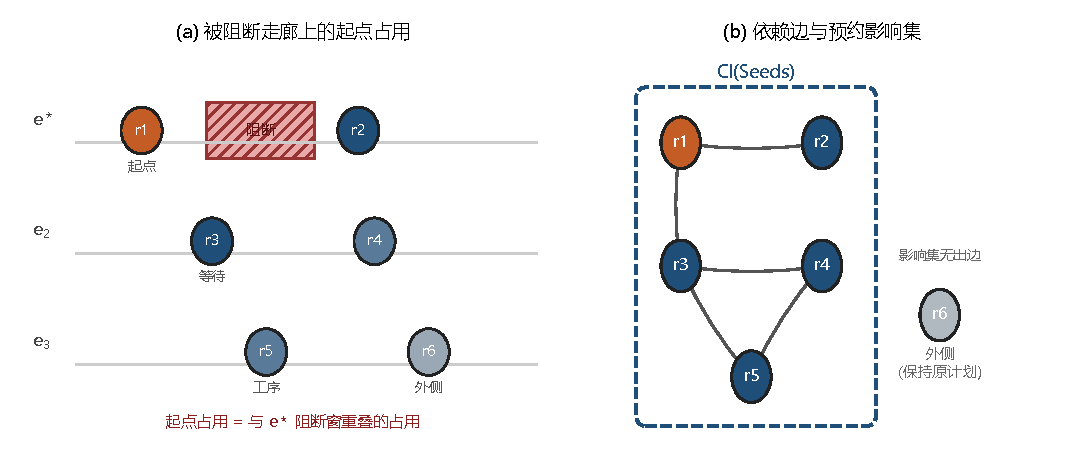
\includegraphics[width=\linewidth]{figures/fig_strc_closure_CN}
\caption{预约影响集的构造示意。
(a)~与走廊阻断窗重叠的占用作为起点；
(b)~沿四类依赖边（让行，以及同车、同工件、同机三类接续）取传递闭包得到
\(\mathrm{Cl}(\mathrm{Src})\)，集外占用保持原计划。}
\Description{两小幅示意图。(a) 时空图上一段阻断窗覆盖若干条占用，
这些占用被标为起点。(b) 从起点沿有向依赖边做传递闭包，得到预约影响集的边界；
边界之外的占用没有来自集内的入边，保持原计划。}
\label{fig:closure}
\end{figure}

按工序依赖图划界的对照，把 \(T_{\mathrm{impact}}\) 映射为允许改写的占用：
凡任务标签属于该影响域且 \(t^e>t_{\mathrm{now}}\) 的占用。
由命题~\ref{prop:miss},B 类上该集合为空。
按预约影响集划界时取 \(U=\mathrm{Cl}(\mathrm{Src})\)。
实验表中二者分别记为 R1 与 R2。

\subsection{包含性}
\label{sec:containment}

\begin{prop}[结构闭合性]
\label{prop:struct}
对任意 \(S\subseteq R\)，在 \(G_R^\circ\) 中不存在边
\(u\to v\) 满足 \(u\in\mathrm{Cl}(S)\) 且 \(v\in R^{\circ}\setminus\mathrm{Cl}(S)\)。
因而，从 \(\mathrm{Cl}(S)\) 出发沿出边无法到达影响集外、尚未结束的占用。
\end{prop}

\begin{proof}
若存在这样的边 \(u\to v\)，则由 \(u\in\mathrm{Cl}(S)\) 知存在尚未结束的起点占用 \(s\) 使
\(s\to^* u\)。拼接 \(u\to v\) 得 \(s\to^* v\)，故按定义~\ref{def:strc} 应有
\(v\in\mathrm{Cl}(S)\)，矛盾。
\end{proof}

命题~\ref{prop:struct} 说明「局部」对应一个图论上闭合的对象：影响集外的占用不是任何
集内占用的直接后继。边集固定后，闭合性即为定义的推论；其物理完备性取决于边集的选取。

\begin{remark}[预约影响集与最小允许改写集合]
\label{rem:minimality}
结构闭合性只说明影响集对所建模的依赖边封闭：集内占用没有指向集外的依赖边。
它既不保证影响集足以恢复可行，也不说明影响集不过大。后者的理由有三。

其一，\textbf{最小允许改写集合依赖于所用的修复程序，而预约影响集不依赖}。
称集合 \(U\) 为最小，须指明「在何种修复能力下 \(U\) 足以恢复可行」。允许改派与改序时的最小 \(U\)，
与只允许改路时的最小 \(U\) 不是同一个集合。预约影响集由 \(G_R\) 唯一确定，与修复程序无关——
因而它在定义上不绑定于某一启发式，也不可能同时是依赖修复程序的最小集。

其二，\textbf{四类边会多纳入不必改写的占用，而已知会漏纳的接壤情形已并入让行边}。
让行边按「同走廊、异车、重叠或接壤」建立，只要重叠即连边，而不判断后者是否\emph{真的}
只能靠等待前者通过——若该处另有旁路，后者改道即可，本不必纳入允许改写的集合；同车后继边同样
可能把延误无法传到的链尾一并纳入。这两处使影响集偏大。
反方向上，半开区间首尾相接（接壤）在排他语义下合法，但前者延后则后者必须让路，
故接壤也按让行边连接；差分试探在 \(\NPairs\) 对上的泄漏为 \ProbeLeaks（\ProbeLeakPairs；
第~\ref{sec:limitations}~节）。这一检验针对的是已知的接壤漏边，并不证明边集完备。

其三，\textbf{实测上影响集并不小}。第~\ref{sec:e6}~节报告，走廊阻断下预约影响集平均覆盖
\(t_{\mathrm{now}}\) 之后尚未结束占用的约 \ClosureAliveFrac；即相对「把决策时刻尚未结束的占用全部纳入改写」这一平凡
上界，影响集少纳入的不足一成。有界修复的节省主要来自\emph{不改写已经结束的占用}与\emph{不重新启动搜索}，
而不是大幅缩小待改写的未来占用；「局部」「有界」不意味着改动范围很小。

「不足一成」是允许改写集合的\emph{规模}之比，不等于改动比例之差。
第~\ref{sec:cheap}~节把上述平凡上界作为一条独立对照(RA)实测后发现，正是这不足一成的
差别，把改动比例从 \ResFracAllFuture\ 降到 \ResFracCheapRtwo（逐格 \RAStabWTL,
\(p=\RAStabP\)），而算法耗时与完工时间几乎不变。

因此，本文给出的是由结构唯一确定、可复现、对依赖边封闭的允许改写集合，
且在本文全部实验中均足以恢复可行；逼近最小允许改写集合是另一个问题，列为后续工作
（第~\ref{sec:future}~节）。
\end{remark}

\begin{prop}[外侧字段不变的充分条件]
\label{prop:outside}
设允许改写的占用集合 \(U=\mathrm{Cl}(S)\)，并设第 1 级改路按第~\ref{sec:level1}~节执行：
(i)~禁行窗已写入路由层；(ii)~对每个 \(r\in R^{\circ}\setminus U\)，将其原字段
\((e,[t^s,t^e),k)\) 预提交到新预约表且预提交成功；
(iii)~仅对 \(U\) 内运输调用路由器生成新占用；(iv)~最终排程通过无冲突校验。
则在恢复后的预约表 \(R'\) 中，每条 \(r\in R^{\circ}\setminus U\) 的走廊、时段与车辆与
\(\mathcal{S}^0\) 一致。此处量词是逐\emph{占用}而非逐任务：一道运输可能一部分占用在 \(U\) 内、
另一部分在外，那时只有集外那部分受本命题保护。
\end{prop}

\begin{proof}
由 (ii)，集外占用在重放开始前已按其原区间写入新表，且未与禁行窗冲突
（否则预提交失败）。步骤 (iii) 只为 \(U\) 内任务提交新占用，不删除或改写已提交的
集外区间。因此，对集外任务标签，新表中的 \((e,[t^s,t^e),k)\) 与预提交值相同，
亦即与 \(\mathcal{S}^0\) 相同。校验通过仅排除新占用与既有占用冲突，不改变已提交字段。
\end{proof}

前提 (i)--(iv) 是第~\ref{sec:level1}~节改路程序的执行条件，可对算法逐条核验，
与 A1--A5 那种模型级假设不同类，故不并入编号假设体系；命题此外依赖
A1（初始排程可行，否则集外原字段之间就可能互相冲突、预提交必然失败）、
A2（已结束占用不回溯）与 A4（走廊排他）。

\begin{remark}[前提 (ii) 与 (iii) 各自会怎样失效]
\label{rem:precommit}
若预提交因「集外占用与禁行窗重叠」失败，则 \(S\) 未能覆盖全部与阻断窗重叠的占用，起点集不完备。
若改路因运输--工序衔接失败而触发第~\ref{sec:scope_escalation}~节扩大范围，则新的允许改写集合
\(U'\supsetneq U\)，命题~\ref{prop:outside} 只对最终未纳入改写的集外占用成立。
扩大范围以可行性优先于改写尽可能少，实验中单独报告。
还有一种失效不在命题的可控范围内，但在实现上容易发生：前提 (iii) 要求路由器\emph{只}
为 \(U\) 内的运输生成新占用。若实现以比占用更粗的单位（例如整道运输、整个工序）决定
是否改路，则 \(U\) 外的占用会被一并改写，前提 (iii) 不再满足，命题的结论随之不成立。
注~\ref{rem:e2b_history} 记录了实现中出现过的这一情形及其修正。
\end{remark}

\subsection{结构可预测性}
\label{sec:structure}

预约影响集的规模由 \(G_R\) 唯一确定，排程与路网给定后没有可调参数。第~\ref{sec:instscale}~节把算例从 \(8\times4\times4\) 放大到
\(\ScaleJobsHi\times\ScaleMachHi\times\ScaleMachHi\)，影响集占比在
\ScaleCloLo--\ScaleCloHi\ 间波动，未随规模增大而上升（该比以全表为分母，其可达上界约为
\ScaleAliveShare；以可改写集合为分母时为 \ScaleCloAliveLo--\ScaleCloAliveHi）。
因而「局部」的范围可以测量，但其规模并不小（注~\ref{rem:minimality}）。

至于\emph{哪种}结构对应更大的影响集，实验结果是否定性的。
本文考察一类只由路网算出、不随当前排程变化的指标：把装卸站与车间其余部分隔开所需切断的最少走廊数，
即装卸站最小割（下称 LU 割），以及漏斗占比；下文把这一族指标称作静态割。
\textbf{影响集规模不由静态割决定}。在自建的同规模布局上，不同边界阻断协议下的
相对规模或落在很窄的带内、或虽有方向但各随机种子上的取值高度重叠；换用一批不由本文设计的路网后，
LU 割与漏斗占比\emph{取值恒定}，而影响集占比在同一张路网上换用三种机器配置
（\(6\)、\(7\)、\(8\) 机）时即明显变化；取值恒定的指标无法解释一个变化的量
（第~\ref{sec:e4}~节）。
这一否定只针对静态割；由于可得的公开路网有限，路网结构与影响集规模的一般关系尚无法判断。
下一个候选刻画应是随排程而变的量，而非纯拓扑量（第~\ref{sec:future}~节）。

%% =====================================================================
\section{预约影响集上的有界修复}
\label{sec:repair}
%% =====================================================================

图~\ref{fig:framework} 总览本节流程：先按预约影响集划定允许改写的占用集合 \(U\)，
再只对集内运输改路、集外保持原计划；仍不可行则扩大 \(U\) 再试。
按工序依赖图划界的对照只替换 \(U\) 的来源；全局重调度对照则在限定时间内重新搜索。
各方法共用同一套走廊路网、时间窗路由与无冲突校验。

\begin{figure}[t]
\centering
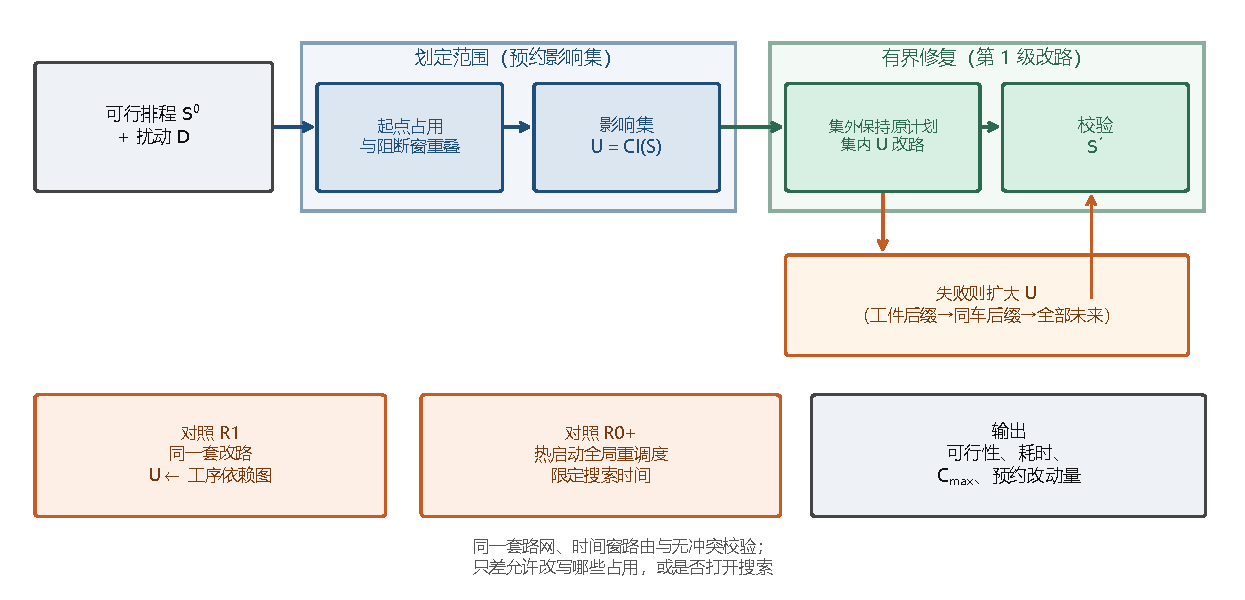
\includegraphics[width=\linewidth]{figures/fig_strc_framework_CN}
\caption{按预约影响集划界的有界修复。
上排：由起点占用得到影响集并改路；中排：失败后扩大允许改写的范围；
下排：按工序依赖图划界的对照与热启动全局重调度对照，以及输出指标。
本图只画方法层的三条路径；毫秒量级内另有三条对照（第~\ref{sec:cheap}~节）。}
\Description{三排流程图。上排：扰动进入后由起点占用得到预约影响集，集内占用允许改写、
集外保持原计划，然后原车辆改路。中排：改路失败时按工件后缀、同车后缀、
全部尚未结束占用的顺序扩大允许改写的集合并重试。下排：两条对照，
一按工序依赖图上的影响域划定范围，一做热启动全局搜索；三条路径汇入同一组输出指标。}
\label{fig:framework}
\end{figure}

\subsection{允许改写、保持原计划与第 1 级改路}
\label{sec:level1}

给定允许改写的占用集合 \(U\)，第 1 级改路保持原车辆指派与机器指派，按原加工顺序重放。
改路以走廊路段（即一次行驶中通过单条走廊的一段，下称路段）为粒度：车辆在 \(t_{\mathrm{now}}\)
前已通过的路段属于已完成占用，原样预提交，改路只从车辆当时所在的节点开始规划；
若粒度粗于路段，就会改写已完成的占用（注~\ref{rem:e2b_history}）。
算法~\ref{alg:replay} 给出这一原语；算法~\ref{alg:strc_repair} 在其外层计算预约影响集，失败时扩大 \(U\)。

\begin{algorithm}[t]
\caption{第 1 级改路重放 \(\textsc{ReplayReroute}\)}
\label{alg:replay}
\begin{algorithmic}[1]
\Require 排程 \(\mathcal{S}^0=(x,\pi,y,R)\)，扰动 \(\mathcal{D}\)，允许改写集合 \(U\)，时刻 \(t_{\mathrm{now}}\)
\Ensure 排程 \(\mathcal{S}'\) 或失败
\State 将 \(\mathcal{D}\) 写入路由层
  \Comment{阻断：禁行窗；通行变慢：重叠段 \(\tau\)}
\State 取空表 \(R'\)
\For{每条不可改写的占用：集外的全部，以及 \(r\in U\) 而 \(r.t^e\le t_{\mathrm{now}}\) 的}
  \State 将原字段 \((e,[t^s,t^e),k)\) 预提交到 \(R'\)
    \Comment{第二类是 A2 规定的已完成占用，遗漏即等于改写它们}
  \If{与阻断窗冲突}
    \State \Return 失败
      \Comment{起点占用未覆盖与窗重叠的占用}
  \EndIf
\EndFor
\For{每条 \(r\in U\)，按原加工顺序}
  \State 从该车辆在 \(t_{\mathrm{now}}\) 所在的节点开始规划 \Comment{已通过的路段已在上一步预提交，不重复提交}
  \State 在当前 \(R'\) 上调用时间窗路由，提交新占用
    \Comment{不改写已经结束的占用}
\EndFor
\State 按 \(\pi\) 推进各机器空闲时刻与各工件就绪时刻
\State 独立校验：无冲突、无禁行窗残留、通行变慢的重叠段时长已吸收、集外字段未改
\If{校验通过}
  \State \Return \(\mathcal{S}'=(x,\pi,y,R')\)
\Else
  \State \Return 失败
\EndIf
\end{algorithmic}
\end{algorithm}

划界那一遍广度优先（定义~\ref{def:strc}）只占耗时的一小部分：一次
\(\textsc{ReplayReroute}\) 还要对 \(|U|\) 个运输段各调用一次时间窗最短路，
实测耗时由后者主导（第~\ref{sec:e3}、\ref{sec:cheap}~节）。
该级不启动种群搜索。第~\ref{sec:e3}~节的对照固定算法~\ref{alg:replay}，只替换 \(U\) 的来源（工序依赖图或预约影响集），
用以把可行率之差归因于划界对象。

\subsection{失败后扩大允许改写的范围}
\label{sec:scope_escalation}

扩大允许改写的范围，本身已有成例。Local Rescheduling~\cite{kuster2007local}
按时间窗逐步放宽直至可行；AOR 则按工件后继与同机后继纳入后续工序
（第~\ref{sec:rw_aor}~节）。本文沿预约依赖边扩大 \(U\)，而不是沿时间窗。
这些步骤用于落实影响集：改路失败时先扩大须改写的占用，而不是立即转为全局搜索。
第~\ref{sec:protocol}~节说明边界消融实验为何必须关闭这一步。

当集外占用保持过紧时，算法~\ref{alg:replay} 可能因运输--工序衔接等校验失败。
此时按下列顺序扩大 \(U\) 并重试同一套改路程序：
(i)~\(U\leftarrow U\cup\{\)当前 \(U\) 内各工序的同工件后缀、尚未结束的占用\(\}\);
(ii)~\(U\leftarrow U\cup\{\)所涉车辆的同车后缀、尚未结束的占用\(\}\);
(iii)~\(U\leftarrow\{\,r\in R:\ r.t^e>t_{\mathrm{now}}\,\}\)（把决策时刻尚未结束的占用全部纳入改写）。
扩大范围后仍是确定性的单遍改路。实验中这一步使全部格恢复可行，算法耗时保持在毫秒至十余
毫秒量级（第~\ref{sec:experiments}~节）。耗时随扰动比例 \(\varphi\) 并非单调变化，
一种可能的解释是两种效应方向相反：比例小时初始影响集偏紧、更常需要扩大范围；比例大时初始 \(U\) 已较宽、
往往一轮即成功，但单轮需要改路的运输更多（结果见第~\ref{sec:scale}~节）。

\subsection{与全局重调度的对照}
\label{sec:vs_r0}

全局重调度对照在相同禁行约束下、在限定时间内以原排程为起点重新搜索（记 R0+）。
内部把 \((x,\pi)\) 编成一条染色体；一次\emph{解码}指：按该染色体的指派与加工顺序，
在已写入禁行窗的预约表上从头为全部运输调用第~\ref{sec:reservation}~节的时间窗路由，
得到新的 \(R\) 与 \(C_{\max}\)。R0+ 重复解码并允许改染色体；第~\ref{sec:cheap}~节的
RD 只解码一次且不改染色体。R0+ 的解码不改写已经结束的占用：这些占用预提交，
只从 \(t_{\mathrm{now}}\) 起排定尚未开始的工序（第~\ref{sec:e5}~节）。
对照取热启动而非从零搜索，以免丢掉原排程已有的指派与路径信息。
R0+ 可改派与改序，因而更可能缩短 \(C_{\max}\)，但算法耗时由预算决定。

有界修复在完工时间上并不优于 R0+。第~\ref{sec:e5}~节表明：R0+ 在最小预算档上已占优，
而 R2 的结果不随预算变化、R0+ 的 \(C_{\max}\) 随预算单调不增，故增加预算也不出现反超。
有界修复的长处在于算法耗时：响应须在毫秒量级时，它能恢复可行；允许秒级停机时，应采用 R0+ 缩短 \(C_{\max}\)。
集外占用的走廊、时段与车辆保持原计划，由命题~\ref{prop:outside} 在其条件下保证。

仅与 R0+ 对照留下一个问题：在毫秒量级的耗时内，按影响集划界是否必要?
为此本文实现三种不按影响集限制范围的做法：全局右移(RS)不判断哪些占用
受影响，只把未完成占用整体后推到阻断结束之后；原染色体重解码(RD)不改染色体，只执行一次固定前缀解码；
\textbf{RA} 把 \(t_{\mathrm{now}}\) 之后尚未结束的占用全部纳入改写，再执行与第~\ref{sec:level1}~节
\emph{完全相同}的改路程序，因而与本文方法只差「允许改写哪些占用」这一项，是唯一能单独检验预约影响集
作用的对照。三者耗时均在毫秒量级，构成有界修复在\emph{同一耗时量级内}的对照，
定义与结果见第~\ref{sec:cheap}~节。

算法~\ref{alg:strc_repair} 把本节与上节合起来写出，与图~\ref{fig:framework} 对应。

\begin{algorithm}[t]
\caption{基于预约影响集的有界修复（第 1 级改路 + 扩大范围）}
\label{alg:strc_repair}
\begin{algorithmic}[1]
\Require 排程 \(\mathcal{S}^0\)，扰动 \(\mathcal{D}\)，时刻 \(t_{\mathrm{now}}\)
\Ensure 排程 \(\mathcal{S}'\) 或失败
\State \(S \gets \mathrm{Src}(\mathcal{D})\);
      \(U \gets \mathrm{Cl}(S)\)
\For{轮次 \(=0,1,2,3\)}
  \State \(\mathcal{S}' \gets \textsc{ReplayReroute}(\mathcal{S}^0,\mathcal{D},U,t_{\mathrm{now}})\)
  \If{\(\mathcal{S}'\) 可行}
    \State \Return \(\mathcal{S}'\)
  \EndIf
  \State 按扩大范围的规则更新 \(U\) \Comment{工件后缀 / 同车 / 全部尚未结束}
\EndFor
\State \Return 失败
\end{algorithmic}
\end{algorithm}

%% =====================================================================
\section{实验}
\label{sec:experiments}
%% =====================================================================

\subsection{协议}
\label{sec:protocol}

\textbf{路网、路由与算例。}
下层路网、时间窗路由与独立校验器固定。扩样矩阵使用\textbf{五个算例}：
小例 \texttt{example\_3x3x2}、拥堵例 \texttt{congested\_8x4x4}，
以及三个 \texttt{S8x4x4} 布局 \texttt{high}、\texttt{funnel} 与 \texttt{mid}。
后三者同规模、同柔性，只差走廊拓扑，因此它们之间预约影响集规模的差异可归因于拓扑而非问题尺寸。
五者分两种来源：前两个是手写布局（小例供逐步核对，拥堵例为哑铃拓扑）；后三个由本文的算例
生成器产生，其参数（工件数 \(\times\) 机器数 \(\times\) AGV 数、拥堵档、异构度 \(h\)、柔性度 \(f\)）
与\textbf{生成随机种子}一并编码在算例文件名中，三者的生成随机种子同为 \(42\)。
\textbf{生成随机种子与下文的运行随机种子相互独立}：前者只决定算例本身，后者决定扰动注入
与搜索过程；两者取值中均含 \(42\)，但并无共用。
\textbf{运行随机种子取十个}，即 \(42\)、\(7\)、\(2024\)、\(99\)、\(123\)、\(13\)、\(1\)、
\(777\)、\(31415\) 与 \(8\)，共 \(\NInst\times\NSeeds=\NPairs\) 个算例--随机种子对，下文每一对称为一「格」。
全文所有逐格比较、胜负计数与配对检验都按（算例，随机种子）这一对键对齐：
同一键下各方法读取同一份初始解、同一段阻断与同一决策时刻。
初始排程由第~\ref{sec:reservation}~节的时间窗路由按加工顺序重放得到，
并通过独立无冲突校验；同一算例--随机种子对下各对照方法共享该初始解。
对 \(\mathcal{S}^0\) 只要求其在扰动前可行。

\textbf{实现与运行环境。}
全部实验为纯 Python 标准库实现，不依赖第三方数值库；下层路网、时间窗路由与独立校验器
复用与静态一体化工作同一份实现。单机单线程运行，不使用并行：Intel Xeon W-1270
（\(8\) 核 \(16\) 线程）、\(64\)\,GB 内存、Windows 10，解释器为 CPython \(3.7.6\)（\(64\) 位）。
因不引入第三方数值库，复现不需要锁定依赖版本；\(3.7\) 是本文实测的解释器，
更高版本未逐一复跑。所有计时结果都在上述单机单线程条件下取得，
更换硬件会使其整体平移，故本文的耗时结论均以\emph{比值}或\emph{量级}形式给出，不依赖绝对毫秒数。

\textbf{代码与数据可用性。}
复现所需材料分三部分：上层有界修复与实验驱动、下层路网与时间窗路由、
算例与扰动输入及全部逐格结果(CSV)。三者连同生成各表各图的脚本一并提交，
审稿期间以\textbf{匿名仓库}形式提供（见投稿系统所附链接，仓库内不含作者身份信息）；
论文接受后转为公开仓库并在永久存档服务上登记 DOI，本节届时补填该 DOI。
每张表与每幅图在仓库中都能追到生成它的脚本与对应的 CSV，
表~\ref{tab:instscale} 所列算例亦随仓库分发。

\textbf{第二批：布局出处外部化。}
上面五个算例的布局都是本文设计的，其中三张同规模布局还同属哑铃一族（彼此只差装卸站
出口与中段的并行通道数，即只差容量、不差几何）。为使布局不由本文决定，另外运行一批
\NPubInst\ 个算例：路网的网格尺寸、装卸站与机器落位、缺失的边这三项逐项转录自
Lyu 等~\cite{lyu2019approach} 附录 A 的布局图，转录结果由脚本与 van Os 配套工具集
所给的机读编码逐字段对账。机器台数因此由布局决定而非由本文选定，为 \(4\) 至 \(8\) 台。
随机种子仍取同样十个，合计 \NPubPairs\ 个算例--随机种子对。两批算例\emph{逐参数同口径}：工件数、
AGV 数、每工件工序数、\(h\)、\(f\) 以及运输/加工时长比的标定目标一律相同，因此两批之差
可唯一归因于布局出处。

该附录共给出六张布局（\(3\) 至 \(8\) 机）。\(3\) 机布局未采用：固定 \(f=0.6\) 在 \(|M|=3\) 时
平均候选机数为 \(1.8<2\)，与「每道工序至少两台候选机」不相容，而为单张布局放宽 \(f\)
会引入额外变量。

其余五张\textbf{只落在 \NPubNets\ 张不同路网上}：\(4\) 机与 \(5\) 机两张共用
同一张 \(4\times 4\) 网格（去掉同一条边），\(6\)、\(7\)、\(8\) 机三张共用同一张
\(5\times 5\) 网格（去掉同两条边）；五者彼此的差别在于机器台数与\emph{落位}，
而非路网几何（原始发布数据即如此组织）。因此第~\ref{sec:e4}~节分析这批
数据时，\textbf{路网几何这一维的独立样本数是 \NPubNets\ 而非 \NPubInst}，机器落位这一维则
有 \NPubInst\ 个；下文的论断均按此划分给出。

该批算例有三处与原始数据不同。\textbf{其一，逐段行驶时间不是原始数据。} Lyu 只为单个示例
算例发表过逐段时长，且其取值并不均匀；附录 A 那批布局的逐段时长从未发表。故这里按
「所有边等权」补齐——它与 van Os 模型里「单步时长为常量」的假设在结构上一致，只是时间单位的
标度不同。因此本批结果不与 Lyu 或 van Os 的参照值比较，仅作为一批非本文设计的拓扑使用。\textbf{其二，装卸站做了合并。} 原布局有分离
的装货站与卸货站，本文只有一个装卸站，故取车辆起始处的装货站作为装卸站，卸货站视为普通
网格节点。\textbf{其三，未采用其工件数据。} 在已实测的公开算例族中，平均运输时长只占平均
加工时长的百分之几，运输几乎不构成争用；若同时采用其工件数据，走廊争用及以其为对象的
全部现象都将无法观察。因此外部化的只有路网。
同一工具集另附的一族布局（其目录标注为 Liu 2023）未纳入本批：这些布局允许对角
移动，而本文的走廊为四邻接；支持对角移动需要修改下层路由，而非算例。

\textbf{扰动。}
除非另注，\(t_{\mathrm{now}}=0.35\,C_{\max}(\mathcal{S}^0)\)。
E1--E3 与 E5 在繁忙走廊上施加单窗阻断；E6 在同一 \(t_{\mathrm{now}}\) 上另加三类扰动；
E4 阻断 LU 割中的走廊（第~\ref{sec:e4}~节）；
扰动规模扫描将未来工序按最早未来预约排序，取前比例 \(\varphi\) 的预约时窗作为微阻断（不合并）。

\textbf{对照方法。}
R1：按工序依赖图上的影响域划界 + 第 1 级改路，全文取 \(\theta=2\)
（该值只影响 A 类扰动下 \(|U_{R1}|\) 的大小；由命题~\ref{prop:miss},B 类上
任何有限 \(\theta\) 都给出空集）；其划界规则取自第~\ref{sec:rw_aor}~节所述的工序级
局部重调度做法，由本文重新实现。逐条对应关系是：「受影响工序集取直接受扰工序，
再沿工件内工序先后关系向后扩张」这一条划界规则对应
AOR~\cite{abumaizar1997rescheduling,subramaniam2003maor}；
而\emph{以跳数 \(\theta\) 截断扩张}、以及\emph{把工序集映射为须释放的走廊预约}
两项由本文写定——原文的设定里没有预约表，这一映射在原文中无对应物；
改路与重放部件则与 R2 共用同一份实现，以保证两者只差划界对象。
因此 R1 是将该划界规则移植到本文预约设定下的对照，其结果反映该规则在此设定下的表现，
而非原方法在其自身设定下的表现；
R2/\STRC：按预约影响集划界 + 第 1 级改路（规模扫描打开失败后扩大范围；E3/E5 关闭这一步）；
R0+：以原排程为起点、在限定时间内重新搜索的全局重调度——遗传算法，种群 \(40\)，
原排程对应的染色体置入初始种群，解码采用与 RD 相同的固定前缀解码（\(t_{\mathrm{now}}\)
之前的占用不可改写）；\emph{不设代数上限与早停阈值}，终止条件只有挂钟预算一项，
预算取值见第~\ref{sec:e5}~节；
RS：全局右移，不按影响集划界且不改路（第~\ref{sec:cheap}~节）；
RD：原染色体重解码，即本实现中耗时最短的全局重算（同节）；
RA：不按影响集限制范围但保留改路，即把 \(t_{\mathrm{now}}\) 之后尚未结束的占用全部纳入改写，其余与 R2 逐项相同，
用于单独检验预约影响集的作用（同节）。
这五条对照按「是否划界 \(\times\) 重算范围」组织：R1 与 R2 只差划界\emph{对象},
RA 与 R2 只差\emph{是否}划界（改路程序完全相同），RS 既不划界又放弃改路而整体后推，
RD 与 R0+ 则重算全局而不按影响集划界，只差搜索多少代。

\textbf{预算口径。}
各方法不在同一预算档上比较：R1、R2、RS、RD、RA 均为一次确定性修复，
运行结束即终止，耗时由算例规模与影响集大小决定而非由预算设定；只有 R0+ 按挂钟预算终止。
因此涉及 R0+ 的结果均为给定预算下的结果；第~\ref{sec:cheap}~节的四法对照才是同一预算档内
（均运行一次即终止）的比较。挂钟耗时按批次报告，不跨批次比较。

\textbf{失败后扩大范围的开关。}
E3 中关闭失败后扩大范围。若开启，R1 可能在扩大到全部尚未结束的占用后恢复可行，
测得的将是扩大规则的回退能力，而不是划界对象的差别。扩大范围本身有效（规模扫描中它使全部格
恢复可行），但它与被测变量无关，故在边界消融中关闭。
其端点即第~\ref{sec:cheap}~节的 RA，该节将其作为独立对照逐格测量代价。

\textbf{两批算例的分工。}
两批并非同一组证据的两次采样，它们回答的问题不同。
主批次回答\emph{现象是否存在、机制能否被单独识别}:B 类扰动下按工序依赖图划界得到空范围而原排程不可行
（第~\ref{sec:e1}~节）、预约影响集对该范围的包含与集外字段的不变性（第~\ref{sec:e2}~节）、
同一套改路程序下只替换划界对象的对照（第~\ref{sec:e3}~节）。这三项都要求完全控制算例参数，
尤其是决定走廊争用是否成立的运输/加工时长比，而公开算例族无法提供这种控制
（第~\ref{sec:limitations}~节局限第 4 条）。第二批回答另一个问题：\emph{这些现象
是否只在本文自选的布局上成立}。它主要用于复现（第~\ref{sec:pubrepro}~节），
不产生新的性能对比结论。

两批合并分析的只有两处。其一是 E4：主批次的三张同规模布局同属一族、几何差异很小，
「指标过粗」与「算例几何差异不足」两种解释无法区分；而外部布局若没有逐参数同口径的
自建对照，也无从判断其影响集占比的变动幅度是否足够大。第二批据此收窄了结构可预测性的结论。
其二是 E5：两批的 E5 协议与参数逐项相同，合并只为增加格数，不改变结论方向。
其余各节的结论由主批次单独给出，第二批只增强其外部效度。

\textbf{统计口径。}
全文有两处推断性检验，均在第~\ref{sec:cheap}~节：R2 与 RA 在改动比例上的差（主检验），
以及 R2 与 RD 在完工时间上的差。二者均采用 Wilcoxon 符号秩检验，双侧，按上述（算例，随机种子）键配对。
按 Holm 法对这两次检验校正后，各自的显著性判断不变；其余各处的逐格胜负、均值与中位数
均为\emph{描述性}统计，不作显著性断言。
该检验配套的效应量报为 Hodges--Lehmann 估计 \(0.037\),\(95\%\) 自助置信区间
\([0.018,\,0.074]\)（百分位法，\(10^4\) 次重采样，固定随机种子）；配对差的均值为
\(\RAStabMean\)，区间 \([0.039,\,0.093]\)。离散度按四分位距报告：改动比例在 R2 上为
\(0.073\)、在 RA 上为 \(0.062\)。
% selfcheck:allow-num 0.073 为 R2 改动比例的四分位距,与 \RAStabMeanNet(剔除恒等格后的平均降幅)同值不同源
由于 \(50\) 格中有 \(18\) 格两法恰好持平，配对差\emph{中位数}的置信区间下端为 \(0\)；
这表明持平格约占胜负计数的三分之一。
其余各批次的表格只给均值、中位与计数，不含区间。

\subsection{E1：工序依赖图给出空范围}
\label{sec:e1}

本节只考察 B 类扰动下两种划界各给出什么范围，不比较修复质量。
表~\ref{tab:e1} 与图~\ref{fig:e1e3}（左）按第~\ref{sec:protocol}~节的走廊阻断协议汇总命题~\ref{prop:miss} 的扩样结果：
在 \(\PassMiss\) 格上，\(T_{\mathrm{impact}}=0\)、起点占用与预约影响集非空、阻断后原排程不可行。

表~\ref{tab:e1} 把三个条件合并计入「三条件通过」一列（逐格结果见 \texttt{e1\_miss.csv} 的
\texttt{n\_T\_impact} 与 \texttt{feasible\_after\_block} 两列）。
其中 \(T_{\mathrm{impact}}=0\) 由定义~\ref{def:task_impact} 对 B 类的约定直接得到；
实质性的结果是后一列恒为假，即原排程\emph{确实}已不可行，两者合起来构成反例。

\begin{table}[t]
\centering
\caption{E1 走廊阻断下工序依赖图给出空范围（每算例 \(\NSeeds\) 个随机种子，共 \(\NPairs\) 对）。
\(|R|\) 为全表占用数，\(\mathrm{Cl}/|R|\) 为预约影响集占全表的比例。均值取多个随机种子的平均。
离散度按四分位距(IQR)报告：逐算例 \(\mathrm{Cl}/|R|\) 的 IQR 在
\EoneFracIqrLo--\EoneFracIqrHi 之间，\(\NPairs\) 对合池的中位为 \EoneFracMed、
极差 \EoneFracMin--\EoneFracMax；可见该比例的算例间差异与随机种子间差异同量级，
不宜只读均值。
「三条件通过」为命题~\ref{prop:miss} 三条件同时成立的格数（\(T_{\mathrm{impact}}=0\)、
起点占用非空、阻断后原排程不可行）。后三行同规模同柔性，只差走廊拓扑。}
\label{tab:e1}
\small
\begin{tabular}{@{}lcccccc@{}}
\toprule
算例 & 随机种子 & 三条件通过 & 均 \(|R|\) & 均 \(|\mathrm{Src}|\)
 & 均 \(|\mathrm{Cl}|\) & \(\mathrm{Cl}/|R|\) \\
\midrule
\texttt{example\_3x3x2}   & 10 & \(10/10\) & \(28.6\)  & \(5.6\)  & \(16.9\) & \(0.59\) \\
\texttt{congested\_8x4x4} & 10 & \(10/10\) & \(85.0\)  & \(15.0\) & \(48.4\) & \(0.57\) \\
\texttt{S8x4x4} (high)    & 10 & \(10/10\) & \(150.5\) & \(15.5\) & \(88.3\) & \(0.59\) \\
\texttt{S8x4x4} (funnel)  & 10 & \(10/10\) & \(149.1\) & \(15.5\) & \(85.4\) & \(0.57\) \\
\texttt{S8x4x4} (mid)     & 10 & \(10/10\) & \(147.6\) & \(15.0\) & \(82.8\) & \(0.56\) \\
\midrule
合计 & \(\NPairs\) & \(\PassMiss\) & --- & --- & --- & --- \\
\bottomrule
\end{tabular}
\end{table}

\(|\mathrm{Cl}|\) 的绝对值随算例变大(\(16.9\)、\(48.4\)、\(82.8\)--\(88.3\))，这是占用总数变多的直接结果；
而 \(\mathrm{Cl}/|R|\) 在五个算例上都落在 \EoneCloLo--\EoneCloHi,\emph{未能}区分三个 \(\texttt{S8x4x4}\) 布局。
这与第~\ref{sec:e4}~节的结论一致：实验没有给出能可靠预测影响集规模的结构指标。
就贡献而言，本节支撑 C1:B 类扰动下按工序依赖图划界得到空范围，而原排程已不可行。

\subsection{E2：包含性}
\label{sec:e2}

结构闭合性(E2a)在 \(\PassClosed\) 格上成立（泄漏 \(=0\)），与命题~\ref{prop:struct} 一致。
第 1 级修复（不扩大范围）在 \(\NPairs/\NPairs\) 格上可行。
集外占用的走廊、时段与车辆逐条不变（E2b，即命题~\ref{prop:outside} 的观测形式）同样在 \(\PassInvar\) 格上
成立（表~\ref{tab:e2}）。

\begin{table}[t]
\centering
\caption{E2 包含性（\(\NSeeds\) 个随机种子/算例；第 1 级可行一列不扩大范围）。
E2a 为结构闭合（泄漏 \(=0\)），
E2b 为集外占用的走廊、时段与车辆\emph{逐条}不变。}
\label{tab:e2}
\small
\begin{tabular}{@{}lccc@{}}
\toprule
算例 & E2a 闭合 & 第 1 级可行 & E2b 集外逐条不变 \\
\midrule
\texttt{example\_3x3x2}   & \(10/10\) & \(10/10\) & \(10/10\) \\
\texttt{congested\_8x4x4} & \(10/10\) & \(10/10\) & \(10/10\) \\
\texttt{S8x4x4} (high)    & \(10/10\) & \(10/10\) & \(10/10\) \\
\texttt{S8x4x4} (funnel)  & \(10/10\) & \(10/10\) & \(10/10\) \\
\texttt{S8x4x4} (mid)     & \(10/10\) & \(10/10\) & \(10/10\) \\
\midrule
合计 & \(\PassClosed\) & \(\NPairs/\NPairs\) & \(\PassInvar\) \\
\bottomrule
\end{tabular}
\end{table}

E2a 与 E2b 含义不同。E2a 是\emph{图上的}性质，由命题~\ref{prop:struct} 保证，
用于检验实现与定义是否一致；E2b 是\emph{修复之后的}性质，检验命题~\ref{prop:outside} 的四条前提
在本文协议下是否成立。其中前提 (ii) 要求集外占用逐条预提交成功；若某条集外占用与禁行窗重叠，
预提交即失败，说明起点占用集不完备（注~\ref{rem:precommit}）。
就贡献而言，E1、E2 与第~\ref{sec:e3}~节的边界消融支撑 C1 与 C2 的\emph{对象层}：预约影响集
由边集唯一确定、对外封闭，且在同一套改路程序下均恢复了可行；划界的净收益由
第~\ref{sec:cheap}~节的 RA 对照给出。

\begin{remark}[实现缺陷被误读为边集缺陷的一例]
\label{rem:e2b_history}
若按\emph{工序}而非\emph{占用}判定是否改路，E2b 仅在 \(24/\NPairs\) 格上通过，
容易被误读为「依赖边集未能覆盖若干弱耦合」。其实际原因是粒度错配：允许改写的是\emph{占用}集合，
而按工序判定时，同一工序的空载段与满载段只要有一段落在影响集内，整道运输就被重新规划。
当只有满载段进入影响集时，同工序的空载段也被改写，而它的任务标签不在允许改写的集合内，
因而被记为集外漂移。\(26\) 个未通过格上的 \(84\) 条漂移占用全部属于这种同工序空载段，
其中 \(71\) 条(\(85\%\))在 \(t_{\mathrm{now}}\) 之前已执行完毕，改写它们同时违反假设 A2。
改为按\emph{段}判定（已执行完或未纳入改写的空载段沿用原计划，
只对落在允许改写集合内的段改路）之后，漂移归零。
可见此时测得的不是边集对物理耦合的覆盖程度，而是命题~\ref{prop:outside} 前提 (iii)
「仅对 \(U\) 内运输调用路由器」在实现上未被满足。
这一误判的一般形式是：把实现与定义之间的粒度错配，误读为模型刻画能力的不足。

\textbf{E2b 无法检出的同类错配。} 按段判定时，一个\emph{跨越}
\(t_{\mathrm{now}}\) 的运输段仍整段重新规划：只要它有一个路段的结束时刻晚于
\(t_{\mathrm{now}}\)，整段的任务标签就进入允许改写的集合，于是它在 \(t_{\mathrm{now}}\)
之前\emph{已通过}的路段也被重排，相当于让车辆回到该段起点重新行驶，违反假设 A2。
E2b 无法检出这一情形，因为这些路段的任务标签位于影响集\emph{内}，不在集外字段的比对范围中。
这一情形由一项独立的已完成占用审计（逐条比对 \(t^e\le t_{\mathrm{now}}\)
的占用）检出：\(\NPairs\) 格中有 \(36\) 格存在此类改写，合计 \(86\) 条。
将粒度细化到\emph{路段}（已通过的路段原样保留，改路只从车辆在
\(t_{\mathrm{now}}\) 时实际所在的节点开始）之后，该审计在全部 \(\NPairs\) 格上归零，
各项通过率不变，\(C_{\max}\) 在 \(6\) 格上改善、无一格变差。
本文各表报告的均为按路段粒度实现的结果；本注中的数字（\(24/\NPairs\)、\(26\) 格 \(84\) 条、\(36\) 格 \(86\) 条）
均来自较粗粒度的实现。
\end{remark}

\subsection{E3：边界消融}
\label{sec:e3}

表~\ref{tab:e3} 与图~\ref{fig:e1e3}（右）固定第 1 级改路并\emph{关闭}失败后扩大范围。
B 类扰动下，R1 在 \(\NPairs/\NPairs\) 格上的允许改写集合为空且不可行，R2 全部可行。

两臂使用同一套改路程序、同一份初始解、同一个 \(t_{\mathrm{now}}\)、同一批随机种子与同一段阻断窗，
\textbf{唯一的差别是允许改写哪些占用}。R1 的允许改写集合为空，第 1 级改路对空集是恒等操作，
原排程保持不变，仍占用被阻断的走廊；因此 R1 的失败来自它判定无需重调度，而非修复质量。
第 1 级改路逐格的耗时中位数为 \(\MsRepairMed\)\,ms、最大 \(\MsRepairMax\)\,ms；表~\ref{tab:e3} 末列
是各算例内 \(\NSeeds\) 个随机种子的均值，两者口径不同，不可直接比较。
就贡献而言，本节把缺口的成因归于划界对象(C2、C3)：同一套改路程序只替换划界对象，恢复可行率即从
\(\FeasRone\) 变为 \(\FeasRtwo\)。

上述反差是否依赖边权标定，另作检验。本文的走廊边权取等权，故按三档非均匀边权
（\texttt{lognormal}、\texttt{lu\_far}、\texttt{split}；数据见 \texttt{weight\_sweep.csv}）
在同一批 \(\NPairs\) 对上重新运行 E1 与 E3：三条件通过与工序依赖图范围为空的结果逐档不变，
R1 仍全格不可行，R2 第 1 级的可行格数依次为 \WeightLogRtwo、\WeightLuRtwo、\WeightSplitRtwo，
唯一不可行的一格出现在 \texttt{split} 档（\texttt{S8x4x4\_high}，随机种子 \(1\)）。
故该反差不依赖等权这一标定。

\begin{table}[t]
\centering
\caption{E3 边界消融（不扩大范围；\(\NInst\) 算例 \(\times\) \(\NSeeds\) 个随机种子）。
miss\_B 指该格上 R1 的允许改写集合为空而 R2 非空。
末列为各算例内 \(\NSeeds\) 个随机种子的均值，与正文逐格中位数口径不同。}
\label{tab:e3}
\small
\begin{tabular}{@{}lccccc@{}}
\toprule
算例 & miss\_B & R1 可行 & R2 可行 & 均 \(|U_{R2}|\) & R2 耗时/ms \\
\midrule
\texttt{example\_3x3x2}   & \(10/10\) & \(0/10\) & \(10/10\) & \(16.9\) & \(0.66\) \\
\texttt{congested\_8x4x4} & \(10/10\) & \(0/10\) & \(10/10\) & \(48.4\) & \(2.84\) \\
\texttt{S8x4x4} (high)    & \(10/10\) & \(0/10\) & \(10/10\) & \(88.3\) & \(3.40\) \\
\texttt{S8x4x4} (funnel)  & \(10/10\) & \(0/10\) & \(10/10\) & \(85.4\) & \(5.09\) \\
\texttt{S8x4x4} (mid)     & \(10/10\) & \(0/10\) & \(10/10\) & \(82.8\) & \(3.96\) \\
\midrule
合计 & \(\NPairs/\NPairs\) & \(\FeasRone\) & \(\FeasRtwo\) & --- & --- \\
\bottomrule
\end{tabular}
\end{table}

\begin{figure}[t]
\centering
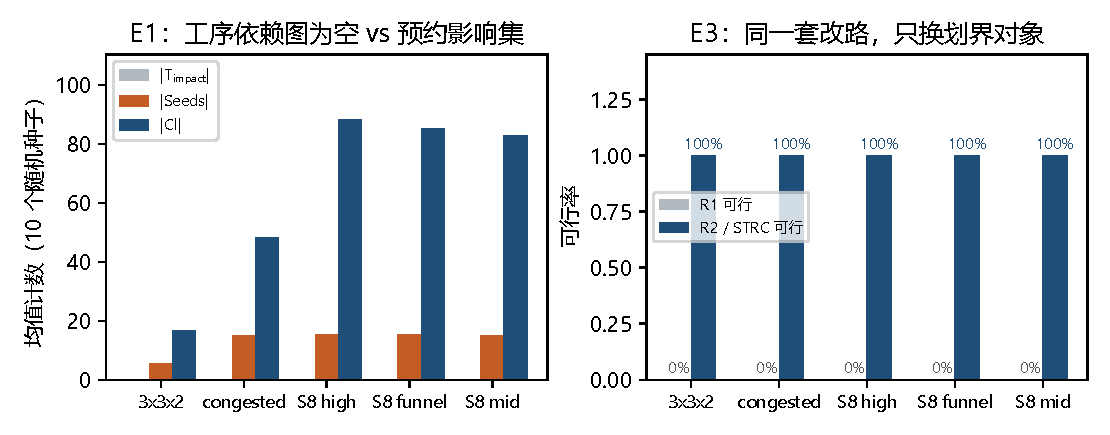
\includegraphics[width=\linewidth]{figures/fig_strc_e1e3_CN}
\caption{E1/E3 扩样可视化（\(\NInst\) 算例 \(\times\) \(\NSeeds\) 个随机种子均值）。
左：工序依赖图上的影响域为空，而起点占用与预约影响集非空；柱高为每算例 \(\NSeeds\) 格
的均值，离散度按四分位距见表~\ref{tab:e1}（\(|\mathrm{Cl}|\) 的 IQR 逐算例在 \(2\)--\(8\)
之间，影响域一组恒为零故无离散度）。
右：同一套改路、只换划界对象时 R1 可行率为 \(0\)、R2 为 \(100\%\)；该幅为逐格计数
（各 \(\NPairs\) 格），故不给出离散度。}
\Description{并排两幅条形图。左幅按五个算例给出工序依赖图影响域、起点占用数与预约影响集规模
三组柱子，影响域一组恒为零，另两组随算例规模上升。右幅给出两种划界的恢复
可行率，按工序依赖图划界一侧为零，按预约影响集划界一侧为百分之百。}
\label{fig:e1e3}
\end{figure}

\subsection{案例甘特图}
\label{sec:case}

\begin{sloppypar}
E1--E3 给出的是跨随机种子的计数与可行率。为在工序时间轴上展示「工序依赖图无法刻画、按预约影响集可以修复」的情形，
图~\ref{fig:case} 取 \texttt{example\_3x3x2}、随机种子 \(42\) 的一例走廊阻断，
协议同 E2/E3：决策时刻取 \(0.35\,C_{\max}\)，繁忙走廊单窗阻断，第 1 级改路、不扩大范围。
\end{sloppypar}

该例上 \(T_{\mathrm{impact}}=\varnothing\)，而 \(|\mathrm{Src}|=6\)、\(|\mathrm{Cl}|=18\)。
图~\ref{fig:case}(a) 为扰动前原排程的机器甘特图：蓝色工序的运输占用落入影响集（将被改路），
灰色工序在影响集外（预提交、保持原计划）；红色虚线为 \(t_{\mathrm{now}}\)，浅红带为阻断时窗。
图~\ref{fig:case}(b) 为修复后：影响集内工序时间轴重排，排程在阻断下恢复可行，
\(C_{\max}:57\to 86\)，耗时亚毫秒级。
本图只说明统计结论对应何种局部改动形态，不用于比较完工时间；
完工时间与全局重调度的权衡见 E5 与扰动规模扫描。

\begin{figure}[t]
\centering
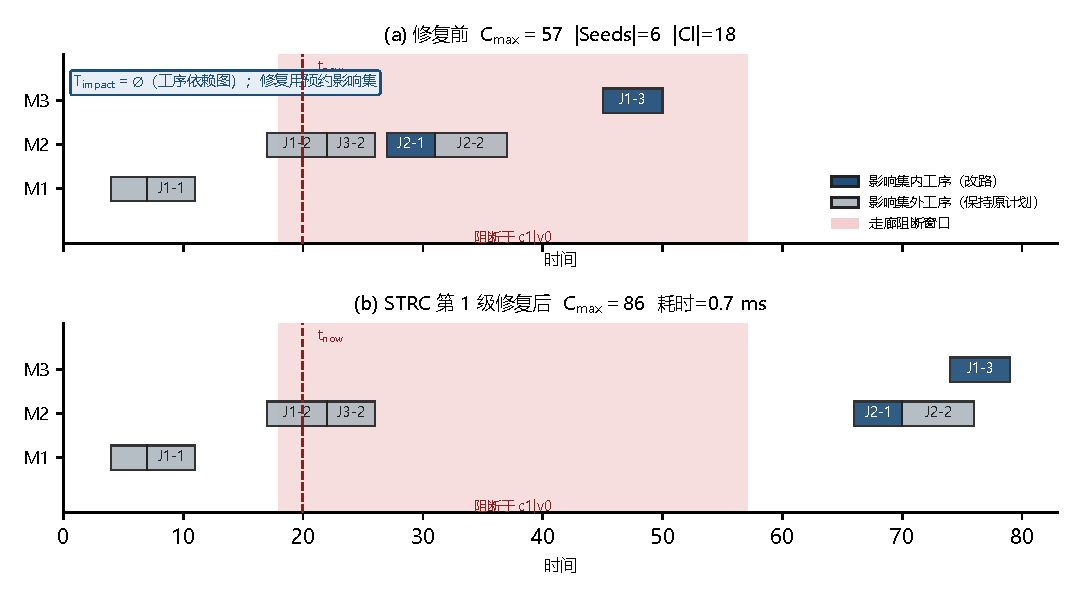
\includegraphics[width=\linewidth]{figures/fig_strc_case_CN}
\caption{案例甘特图（\texttt{example\_3x3x2}，随机种子 \(42\)）。
(a)~阻断前原排程，按是否属于 \(\mathrm{Cl}\) 着色；
(b)~第 1 级修复后。工序依赖图上的影响域为空；蓝色工序对应影响集内运输被改路。
本图仅示意局部改动的形态。}
\Description{上下两幅机器甘特图。(a) 阻断前的原排程，条块按其运输占用是否落在
预约影响集内着蓝灰两色，一条竖直红虚线标出决策时刻，一条浅红竖带标出阻断时窗。
(b) 修复后的排程，蓝色条块的时间轴被重排，灰色条块位置不变，完工时间由 57 增至 86。}
\label{fig:case}
\end{figure}

\subsection{E4：结构（探索）}
\label{sec:e4}

阻断 LU 割中的走廊时，funnel 与 high 的预约影响集占比随随机种子波动（表~\ref{tab:e4}）。
方向上 funnel 更高（中位数 \(0.254\) 对 \(0.204\)，均值 \(0.244\) 对 \(0.229\)），
但\emph{两组取值高度重叠}:funnel 落在 \([0.180,0.309]\),high 落在
\([0.156,0.372]\)，后者的区间完全包含前者，且单个随机种子即可使方向反转
（随机种子 \(2024\) 上 high 的 \(0.372\) 高于 funnel 的 \(0.296\)）。
在五个随机种子、两个布局上，这一差距不足以支撑任何结论。
第~\ref{sec:e1}~节按繁忙走廊阻断协议在三个同规模布局上得到的
\(\mathrm{Cl}/|R|\) 亦落在 \EoneCloLo--\EoneCloHi 的窄带内，同样未能区分布局。

\textbf{外部布局用于区分负结果的成因。}
三张同规模布局同属哑铃一族，几何差异很小（见表~\ref{tab:e4pub}：节点数 \(9\)--\(11\)、
走廊数 \(8\)--\(12\),LU 割仅取 \(1\) 或 \(2\)）；「指标过粗」与
「算例几何差异不足」两种解释在这些布局上无法区分。第~\ref{sec:protocol}~节的
第二批算例用于区分二者（表~\ref{tab:e4pub}）。

\textbf{外部布局上的结果与预期方向相反。}
这批算例在路网几何上只有 \NPubNets\ 个独立样本（第~\ref{sec:protocol}~节），故只用于考察机器配置这一维。
在\emph{同一张} \(4\times 4\) 路网上，只把机器台数与落位从 \(4\) 机换成 \(5\) 机，
影响集占比中位即由 \PubCloHi\ 落到 \PubCloLo，极差 \PubCloSpread；
同一张 \(5\times 5\) 路网上换三种机器配置（\(6\)、\(7\)、\(8\) 机），极差 \PubCloSpreadBig。
作为对比，\emph{逐参数同口径}的三张自建布局（三张\emph{不同}的路网）
的占比只落在 \SelfCloLo--\SelfCloHi，极差 \SelfCloSpread。
即\textbf{路网固定而机器配置变动时，影响集占比的变化幅度可以超过更换三张不同路网时的幅度}：
在 \(4\times 4\) 路网上约为四倍，在 \(5\times 5\) 路网上约为一点五倍。
这一比较并不对称：外部一侧同时改变了机器台数与落位，自建一侧只改变路网；且三张自建布局的几何差异很小，
\SelfCloSpread\ 只是「更换路网」幅度的\emph{下界}。因此它表明机器配置这一维不可忽略，
但不表明其效应大于路网几何。

\textbf{仅由路网决定的最小割无法解释影响集规模。}
在这 \NPubInst\ 个外部算例上，\textbf{LU 割恒为 \(2\)、漏斗占比恒为 \(0\)}：
两张路网都把装卸站放在网格角点，而四邻接网格的角点恰有两条出边，故该割值固定为 \(2\)；
同一工具集另附的那族布局（因允许对角移动未纳入本批）把装卸站放在网格边中点，出边数为 \(3\)。
\textbf{可见该指标在实际布局上只取少数几个由装卸站网格位置决定的离散值}，不随几何连续变化。
更重要的是，\textbf{这两个指标在上述全部变动中保持不变}，而被解释的量变化了
\PubCloSpread；取值恒定的指标无法解释一个变化的量。第三个指标（每节点走廊数）在整批上只取两个值（\(23/16\) 与
\(38/25\)），同样不足以解释组内的变化。

据此，\textbf{在这 \NPubInst\ 个外部算例与三张自建布局上，静态割不能解释影响集规模}。
这一族指标原本针对哑铃布局中可调的装卸站出口瓶颈而设计，在实际布局上退化为常量，不具备解释力。
替代方向由此指向需求侧：决定影响集规模的可能不是路网\emph{能}提供多少条通路，而是
\emph{需求的空间分布}；具体的候选量见第~\ref{sec:future}~节。
本节为探索性的负结果，不对应任何一项贡献。

\begin{table}[t]
\centering
\caption{E4 预约影响集占比 \(\mathrm{Cl}/|R|\)（阻断 LU 割中的走廊；随机种子 \(42,7,2024,99,123\)）。
本表算例为 \(12\) 工件 / \(8\) 机 / \(12\) 辆车、运输与加工时长比标定为 \(4.0\)。
\textbf{该口径与表~\ref{tab:e4pub} 不同}（后者为 \(8\) 工件 / \(4\) 机 / \(4\) 辆车、
比值 \(1.0\)、十个随机种子），两表虽共用 \texttt{funnel}/\texttt{high} 这两个布局名，
\emph{数值不可跨表比较}；表~\ref{tab:e4pub} 内部才是同口径对照。}
\label{tab:e4}
\small
\begin{tabular}{@{}lcccccc@{}}
\toprule
布局 & \(42\) & \(7\) & \(2024\) & \(99\) & \(123\) & 中位数 \\
\midrule
funnel & \(0.254\) & \(0.181\) & \(0.296\) & \(0.309\) & \(0.180\) & \(0.254\) \\
high & \(0.156\) & \(0.204\) & \(0.372\) & \(0.229\) & \(0.184\) & \(0.204\) \\
\bottomrule
\end{tabular}
\end{table}

\begin{table}[t]
\centering
\caption{E4 自建布局与外部布局的对照（阻断 LU 割中的走廊，十个随机种子；\(\mathrm{Cl}/|R|\) 取中位数）。
全表逐参数同口径，只差路网与机器配置。\textbf{外部算例只落在 \NPubNets\ 张路网上}
（\(\mathrm{N}_1\):\(4\times 4\) 去一条边；\(\mathrm{N}_2\):\(5\times 5\) 去两条边），
组内各行\emph{共享同一路网}，只差机器台数与落位；「极差」一列按\emph{组内}给出，
\(\mathrm{N}_1\) 组仅 \(2\) 行、自建组 \(3\) 行，故组间极差之比只作量级参考。
LU 割与漏斗占比在整个外部批次上\emph{取值恒定}。}
\label{tab:e4pub}
\small
\begin{tabular}{@{}llcccccc@{}}
\toprule
出处/路网 & 算例 & 机器 & 节点/走廊 & LU 割 & 漏斗占比 & \(\mathrm{Cl}/|R|\)
 & 组内极差 \\
\midrule
外部 \(\mathrm{N}_1\) & \texttt{LyuL2} & \(4\) & \(16/23\) & \(2\) & \(0\) & \(0.512\) & \\
外部 \(\mathrm{N}_1\) & \texttt{LyuL3} & \(5\) & \(16/23\) & \(2\) & \(0\) & \(0.305\)
  & \(\PubCloSpread\) \\
\cmidrule{1-8}
外部 \(\mathrm{N}_2\) & \texttt{LyuL4} & \(6\) & \(25/38\) & \(2\) & \(0\) & \(0.385\) & \\
外部 \(\mathrm{N}_2\) & \texttt{LyuL5} & \(7\) & \(25/38\) & \(2\) & \(0\) & \(0.422\) & \\
外部 \(\mathrm{N}_2\) & \texttt{LyuL6} & \(8\) & \(25/38\) & \(2\) & \(0\) & \(0.460\)
  & \(\PubCloSpreadBig\) \\
\midrule
自建 & \texttt{high} & \(4\) & \(10/10\) & \(2\) & \(0.286\) & \(0.497\) & \\
自建 & \texttt{funnel} & \(4\) & \(9/8\) & \(1\) & \(0.286\) & \(0.491\) & \\
自建 & \texttt{mid} & \(4\) & \(11/12\) & \(2\) & \(0.286\) & \(0.446\)
  & \(\SelfCloSpread\) \\
\bottomrule
\end{tabular}
\end{table}

\subsection{E5：与全局重调度的权衡}
\label{sec:e5}

本小节检验是否存在\emph{交叉点}，即预算紧时有界修复占优、预算放宽后热启动全局重调度
在 \(C_{\max}\) 上反超。\textbf{在所测的 \(0.2\)--\(2\)\,s 区间内不存在这样的交叉点，
且该结论可向更大预算外推}。这由两条曲线的形状决定：R2 是单次确定性计算，
同一格的三个预算档共用同一次计算结果，\(C_{\max}\) 不随预算变化；R0+ 报告的是逐代最优，
随机种子固定后增加预算只是让同一条搜索轨迹多运行若干代，\(C_{\max}\) 单调不增。
因此两者的次序一旦在\emph{最小}预算档上确定，增加预算便不会使其反转，
只需考察最小档：在 \(\EfiveCells\) 个算例--随机种子格中，R0+ 在 \(\EfiveWinMin\) 格严格
更优、\(\EfiveTieMin\) 格持平，无一格更差。

上述单调性只能向\emph{更大}预算外推。在更低预算一侧，次序可能反转：R0+ 每评估一个候选至少需要一次解码
（同批 \(\MsRedecode\)\,ms，第~\ref{sec:cheap}~节），按其种群规模，仅评估初始种群所需的
挂钟时间已与最小预算档同量级，而 R2 在同批只需 \(\MsCheapRtwo\)\,ms 且全部格可行；
预算再收紧时 R0+ 将无法完成一代评估。所测最小档恰位于这一边界附近，更小的预算未作扫描。

表~\ref{tab:e5} 与图~\ref{fig:e5} 给出其中自建布局的一半：两个算例 \(\times\) 随机种子
\(\{42,7,2024\}\) \(\times\) 预算 \(\{0.2,1,2\}\)\,s。第~\ref{sec:pubrepro}~节在两个\emph{外部}
布局上以同一份代码、同一组参数执行同一协议；两批合计 \(\EfiveInst\) 个算例、
\(\EfiveCells\) 个算例--随机种子格、\(\EfivePts\) 个预算点，逐点 R0+ 胜/持平/负为
\(\EfiveWLT\)，上述单调性与 R2 结果不随预算变化两点已在 \(\EfiveCells\) 个格上逐格核对。
\(\EfivePts\) 个点并非独立样本（算例只有 \(\EfiveInst\) 个），故本节不作显著性检验；
交叉点不存在这一结论由单调性给出，在算例维度上则只在这 \(\EfiveCells\) 个格上得到验证。

\begin{table}[t]
\centering
\caption{E5 与不改写已结束占用的热启动全局重调度（\(3\) 个随机种子均值）。
「改动比例」为被改写的占用占全表之比。本表只含自建布局，共 \(2\) 算例 \(\times\) \(3\) 随机种子
\(\times\) \(3\) 预算点，独立格数 \(6\)；两列 \(C_{\max}\) 相比，R0+ 在每个预算点上更优。
与外部布局批次（第~\ref{sec:pubrepro}~节）合计为 \(\EfiveCells\) 格 \(\EfivePts\) 点，
逐点胜/持平/负为 \(\EfiveWLT\)。R2 结果不随预算变化，故每个算例的三行共用同一个 R2 结果。}
\label{tab:e5}
\small
\begin{tabular}{@{}lcccc@{}}
\toprule
算例 & 预算/s & R0+ \(C_{\max}\) & R2 \(C_{\max}\) & 改动比例 R0+ / R2 \\
\midrule
\multirow{3}{*}{\texttt{congested\_8x4x4}}
 & \(0.2\) & \(279.3\) & \(299.0\) & \(0.61\) / \(0.57\) \\
 & \(1.0\) & \(276.0\) & \(299.0\) & \(0.61\) / \(0.57\) \\
 & \(2.0\) & \(275.7\) & \(299.0\) & \(0.61\) / \(0.57\) \\
\addlinespace[2pt]
\multirow{3}{*}{\texttt{example\_3x3x2}}
 & \(0.2\) & \(78.3\)  & \(88.7\)  & \(0.60\) / \(0.60\) \\
 & \(1.0\) & \(78.3\)  & \(88.7\)  & \(0.60\) / \(0.60\) \\
 & \(2.0\) & \(78.3\)  & \(88.7\)  & \(0.60\) / \(0.60\) \\
\bottomrule
\end{tabular}
\end{table}

\begin{figure}[t]
\centering
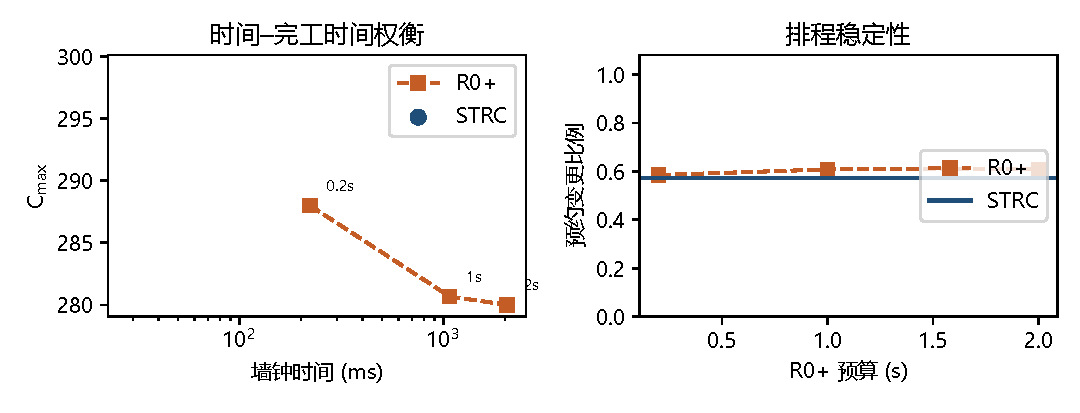
\includegraphics[width=\linewidth]{figures/fig_strc_e5_CN}
\caption{E5：不改写已结束占用的 R0+ 预算扫描与有界修复结果（\texttt{congested\_8x4x4}, \(3\) 个随机种子均值）。
左：算法耗时--\(C_{\max}\)，两条曲线不相交；右：占用改动比例，两法均约为 \(0.6\)。}
\Description{并排两幅图。左幅横轴为对数刻度的算法耗时、纵轴为完工时间：
不改写已结束占用的热启动全局重调度随预算略降，有界修复是左上方的一个单点，
两者不相交，全局重调度在每个预算点上都略低。右幅为占用改动比例，
两法均约为 0.6。}
\label{fig:e5}
\end{figure}

有界修复的完工时间在全部预算区间上均较差，但算法耗时低两至三个数量级（以第 1 级改路的 \(\MsRepairMed\)\,ms
对比 \(0.2\)--\(2\)\,s 预算，见图~\ref{fig:e5} 左）。这一耗时差来自单遍改路、不重新启动搜索，
\emph{并非}来自影响集划界；第~\ref{sec:cheap}~节以耗时相同的 RA 对照证实了这一点。
两者的改动比例同为 \ResFracRtwo\ 量级，改写量的比较见第~\ref{sec:cheap}~节与 RA 的对照。
要求毫秒量级响应时，有界修复能够恢复可行；允许秒级停机时，不改写已结束占用的热启动全局重调度在完工时间上占优。

本表的 R0+ 采用第~\ref{sec:vs_r0}~节的固定前缀解码，不改写已经结束的占用。
对已结束占用是否被改写的检查表明，小例与拥堵例各 \(9\) 个预算点的越界数均为 \(\RzeroPastLo\)；
当同一工件的后道工序已由车辆运出、前道工序仍需重新定时时，R0+ 强制沿用原车辆，只重规划 \(t_{\mathrm{now}}\) 之后的尾段，
从而保留已执行的空载前缀。有界修复在相同各格上的越界数同样为零。
因此，两者的完工时间差距中不包含「改写已经结束的占用」带来的部分，
剩余差距来自全局改派与改序相对单遍改路的优势。
因此，预约影响集的作用不体现在完工时间上，其适用场景是要求毫秒量级响应的恢复。

%% 标题里不放 \(\times\):它会进 PDF 书签,hyperref 无法处理数学模式。
\subsection{E6：扰动类型与划界对象的交叉}
\label{sec:e6}

E1--E3 只考察了走廊阻断一种扰动。本小节展开扰动类型这一维，在同一 \(\NPairs\) 对上另加
走廊通行变慢、车辆故障与机械臂故障三类，结果见表~\ref{tab:e6}。

\textbf{测量内容。} 划界方面，四类扰动均报告工序依赖图上影响域的规模、预约影响集的规模，以及后者是否包含前者。
修复方面，四类扰动均执行修复。B 类仍只改路：阻断把禁行窗写入预约表；通行变慢在窗内按倍率
\(\tau_{\mathrm{mult}}=2\) 降低通行进度，窗外仍按原 \(\tau\) 通行，走廊保持可通行。
A 类额外允许换车或改派，不改变加工顺序；是否扩大允许改写的范围不影响其动作集合。

\begin{table}[t]
\centering
\caption{E6 扰动类型 \(\times\) 划界对象（\(\NPairs\) 对/类，共 \(200\) 次测量；
其中两类 B 扰动按构造给出同一起点集，故\emph{独立}划界测量为 \(150\) 次，见正文第三点）。
\(|R^{\circ}|\) 为 \(t_{\mathrm{now}}\) 之后尚未结束的占用数。
「R1 为空」即按工序依赖图划界判该扰动无需重调度的格数。
末列不扩大范围：B 类为第 1 级改路，A 类为换车或改派。}
\label{tab:e6}
\small
\begin{tabular}{@{}llccccc@{}}
\toprule
扰动 & 类 & R1 为空 & 均 \(|U_{R1}|\) & 均 \(|\mathrm{Cl}|\)
 & \(\mathrm{Cl}/|R^{\circ}|\) & R2 可行 \\
\midrule
走廊阻断   & B & \(50/50\) & \(0.0\)  & \(64.4\) & \(0.92\) & \FeasESixBlock \\
走廊通行变慢 & B & \(50/50\) & \(0.0\)  & \(64.4\) & \(0.92\) & \FeasSlow \\
车辆故障   & A & \(0/50\)  & \(31.1\) & \(60.6\) & \(0.85\) & \FeasESixAgv \\
机械臂故障 & A & \(0/50\)  & \(42.8\) & \(65.9\) & \(0.94\) & \FeasESixRa \\
\bottomrule
\end{tabular}
\end{table}

四点结果。第一，\textbf{A/B 二分在 \(150\) 次\emph{独立}划界测量上无一例外}（两类 B 扰动共用同一起点集，见第三点）：两类 B 扰动按工序依赖图划界
全部为空，两类 A 扰动全部非空。第二，\textbf{在全部 \(100\) 次 A 类测量上
\(U_{R1}\subseteq\mathrm{Cl}\)}，即改用预约影响集划界在 A 类上不会\emph{遗漏}
工序依赖图已纳入的占用。包含在 \(\StrictlyLarger\) 格上是严格的，其余 \(13\) 格两者相等。
机械臂故障一行的包含\emph{按构造}成立：定义~\ref{def:seeds}(c) 的起点规则沿工件链
取整条后缀，而 \(U_{R1}\) 以 \(\theta=2\) 截断（第~\ref{sec:protocol}~节），故该行只验证实现与定义一致；
车辆故障一行的包含则是实测结果。
代价是允许改写的集合平均变大：车辆故障 \(31.1\to 60.6\)，机械臂故障 \(42.8\to 65.9\)。
第三，\textbf{通行变慢与阻断的划界结果逐格相同}，在全部 \(50\) 对上影响集规模一致。
这是因为二者的起点规则相同（与失效时窗重叠、尚未结束的占用），按构造给出同一个预约影响集；
该行表明按工序依赖图划界对通行变慢同样给出空范围。
第四，\textbf{修复方面四类扰动均全部可行}，逐类结果见表~\ref{tab:e6} 末列，通行变慢与阻断口径相同。
通行变慢只按倍率缩放与窗重叠部分的进度，走廊保持可通行，
因此它与「整段禁行后绕路」在物理上仍有区别；第 1 级改路即全部可行，未触发扩大范围。
车辆故障采用换车，机械臂故障采用改派。

\textbf{这张表也给出了影响集规模的实测}（注~\ref{rem:minimality}）。
走廊阻断下预约影响集覆盖 \(t_{\mathrm{now}}\) 之后尚未结束占用的约 \(\ClosureAliveFrac\)；
相对「把尚未结束的占用全部纳入改写」这一平凡上界只少纳入不足一成。
第~\ref{sec:e1}~节按全表统计的 \(\mathrm{Cl}/|R|\) 落在 \EoneCloLo--\EoneCloHi，
与此并不矛盾：全表还包含 \(t_{\mathrm{now}}\) 之前已执行完毕、不可改写的约一半占用。
就贡献而言，本节把 C1 与 C2 的结论从一种扰动推广到四种。

\subsection{E7：毫秒量级内的对照}
\label{sec:cheap}

E5 的对照是热启动种群搜索，预算 \(0.2\)--\(2\)\,s。仅以它为对照会留下一个问题：
\emph{「低两至三个数量级」这一结果，有多少来自预约影响集，又有多少只是因为对照方法耗时更长?}
本节补充耗时介于有界修复与热启动种群搜索之间的对照，并加入一个仅改变允许改写范围的对照。

\begin{itemize}[leftmargin=1.5em,itemsep=0.25em]
\item \textbf{RS（全局右移）。} 不改路径、不改指派、不改加工顺序，把未完成占用整体后推
一个延迟 \(\Delta\),\(\Delta\) 取到刚好让受阻走廊上所有可动的占用落到阻断窗之后。
不改写已经结束的占用（\(t^e\le t_{\mathrm{now}}\) 不可动），与 R2 相同；
由于是统一平移，所有时间间隔保持不变或变大，而全部约束都是「\(\ge\)」型，
无需重新路由即得可行解。它代表「\emph{不按影响集划界}」的一端，且完全不改路
（第~\ref{sec:rw_aor}~节）。
\item \textbf{RD（原染色体重解码）。} 保持机器指派与加工顺序，在已写入阻断的路由层上
执行与 R0+ 相同的固定前缀解码。它是本文实现中\emph{耗时最短的全局重算}；由于不改变染色体，其耗时比 R0+ 短，
改派与改序的自由度也更小。
\item \textbf{RA（不按影响集限制范围，但保留改路）。} 把 \(t_{\mathrm{now}}\) 之后\emph{尚未结束}的占用全部纳入改写，
再执行与 R2 \emph{完全相同}的改路重放。它代表「不按影响集划界」的另一端：与 RS 不同，它保留了
改路，因而与 R2 的唯一区别是允许改写的占用集合。两者使用同一套改路程序，都不改写已经结束的占用，且面对同一段阻断。
因此它是本文\emph{唯一}能单独隔离预约影响集作用的对照，两法之差不含改路程序、协议或实现的贡献。
RA 的允许改写集合已是最大，无需失败后扩大范围。
\end{itemize}

E3 比较的是两种\emph{不同}的划界对象（工序依赖图与预约影响集），而 RA 回答的问题是：
\emph{是否需要按影响集限制改写范围}。

\begin{table}[t]
\centering
\caption{E7 毫秒量级内对照（\(\NPairs\) 对，协议与 E3 相同：繁忙走廊单窗阻断、
\(t_{\mathrm{now}}=0.35\,C_{\max}^{0}\)、R2 不扩大范围）。四法均 \(\NPairs/\NPairs\) 可行。
「已结束占用越界」为改写了已结束占用的格数；「允许改写」为该方法纳入改写的占用占 \(t_{\mathrm{now}}\)
之后尚未结束占用的比例；末列为该方法对 R2 的 \(C_{\max}\) 胜负。RA 与 R2 只差允许改写哪些占用，
故这两行之差可全部归因于预约影响集。本表\emph{不可}与表~\ref{tab:e5} 直接比较，后者只含两个算例。}
\label{tab:cheap}
\small
\begin{tabular}{@{}lcccccc@{}}
\toprule
方法 & 已结束占用越界 & ms（中位）& 平均退化 & 改动比例 & 允许改写 & 对 R2 赢/平/输 \\
\midrule
RS 全局右移      & \ShiftBad     & \MsShift    & \(58.8\%\) & \ResFracShift    & ---   & \(7/16/27\) \\
RD 重解码        & \RedecodeBad  & \MsRedecode & \(49.0\%\) & \ResFracRedecode & ---   & \(22/14/14\) \\
RA 不按影响集划界 & \ShiftBad     & \MsAllFuture & \(49.9\%\) & \ResFracAllFuture & \(1.00\) & \(0/46/4\) \\
R2 有界修复      & \ShiftBad     & \MsCheapRtwo & \(49.8\%\) & \ResFracCheapRtwo & \ClosureShareMean & --- \\
\bottomrule
\end{tabular}
\end{table}

表~\ref{tab:cheap} 给出四条结果。

\textbf{其一，在给出可行方案的各法中，唯一比有界修复更快的是全局右移，
但它在完工时间与改动比例上均较差。}（按工序依赖图划界的 R1 更快，但其可行率仅为 \FeasRone，
不构成候选方法。）
RS 只需 \MsShift\,ms，约为 R2 的一半；代价是完工时间平均退化 \(58.8\%\)（R2 为
\(49.8\%\)），逐格对比为 \WinVsShift（R2 赢/平/输），且改动的占用更多
（\ResFracShift\ 对 \ResFracCheapRtwo），因为统一平移改变了每一条尚未结束占用的时刻。
若要使右移\emph{有选择}，即只推迟真正受影响的车辆而其余保持不变，就必须先
确定哪些占用受影响，而这正是本文划定的范围。\textbf{右移无需按影响集划界，正是因为
它放弃了选择。}

\textbf{其二，耗时最短的全局重算仍比有界修复慢。} RD 的耗时中位数为
\MsRedecode\,ms，是 R2 的 \RedecodeRatio\ 倍。这一结果与搜索配置无关：任何基于解码的搜索，
每评估一个候选至少需要一次解码。因此 E5 中「低两至三个数量级」\emph{并非}
由于对照方法耗时过长；将对照换成同一实现中耗时最短的全局重算，有界修复仍然更快。

\textbf{其三，在不改写已结束占用的前提下，RD 与 R2 的完工时间在本样本上无法区分，但 RD 改动更多。}
全表中 R2 对 RD 为 \WinVsRedecode（赢/平/输），平均退化 \(49.8\%\) 对 \(49.0\%\)。这一差别不显著：
配对差均值 \(+0.006\)，自助 \(95\%\) 区间 \([-0.007,\,0.019]\) 包含 \(0\);Wilcoxon 符号秩
双侧 \(p=0.12\)（非零差 \(36\) 格）；\(C_{\max}\) 比值均值 \(0.997\)，区间 \([0.988,\,1.007]\) 亦包含 \(1\)。
故两者在完工时间上未观察到差异。
RD 的已结束占用越界数为 \RedecodeBad：当后道工序已由车辆运出时，RD 强制沿用原车辆，只重规划决策时刻之后的尾段，
从而保留已执行的空载前缀。因此 RD 在逐格计数上的微弱优势来自同一染色体下全局改路相对单遍改路的优势，
而非改写已结束的占用。RD 的改动比例为 \ResFracRedecode，高于 R2 的
\ResFracCheapRtwo，即按影响集划界的一方改写更少。

\textbf{其四，改写量的减少只能由 R2 与 RA 的对比得出，且只体现为稳定性。} RA 与 R2 的唯一区别是允许改写的占用集合，因此这一对
结果直接给出按影响集划界的净收益。预约影响集平均只比平凡上界少纳入 \(1-\ClosureShareMean\)
的尚未结束占用（逐格为 \ClosureShareLo--\(1.00\)；在取值为 \(1.00\) 的 \(6\) 格上，影响集\emph{等于}
全部尚未结束占用，两法结果相同）。这不足一成的差别使改动比例从 \ResFracAllFuture\ 降至
\ResFracCheapRtwo：平均降低 \RAStabMean，中位数降低 \RAStabMed，逐格为 \RAStabWTL（R2 更稳/持平/更差），
Wilcoxon 符号秩双侧 \(p=\RAStabP\)。

剔除上述 \(6\) 个恒等格后为 \(44\) 格，逐格为 \RAStabWTLNet，平均降低 \RAStabMeanNet
（两种口径下 Wilcoxon 的非零差格数均为 \(32\)），即按 \NPairs\ 格报告的降幅偏保守。
降低的方向高度一致，但\emph{幅度不大}；在唯一的反例格上，R2 多改写了 \(0.007\)。
与此同时，两法的算法耗时几乎相同（\MsCheapRtwo\ 对 \MsAllFuture\,ms），
完工时间也几乎相同（比值均值 \RACmaxRatio，逐格 R2 赢/平/输为 \WinVsAllFuture，从未更差，
最优的一格为 \RACmaxLo）。

上述三项结果需要合并解读。\textbf{耗时相同，说明毫秒量级的响应来自单遍改路、不重新启动搜索，而非来自预约影响集
（结果见表~\ref{tab:cheap}；单遍改路本身是既有做法，见表~\ref{tab:position}）。
完工时间相同，说明影响集不是一种优化手段。
改动比例显著更低，说明划界实现的正是命题~\ref{prop:outside} 所保证的性质：集外占用的走廊、时段与车辆保持不变。}
影响集的作用在于\emph{标明哪些占用无需改写}。
影响集排除的占用越多，降幅越大；但被排除的占用本身只能解释
\(\ResFracAllFuture-\ResFracCheapRtwo\) 这一差距的一部分，其余来自允许改写集合缩小后改路结果的变化。
在影响集接近全部尚未结束占用的算例上（\texttt{congested\_8x4x4}，允许改写占比 \(0.94\)），
降幅仅为 \(0.010\)；而在排除较多占用的算例上(\texttt{S8x4x4\_mid},\(0.91\))，降幅达 \(0.118\)。
% selfcheck:allow-num 0.91 为该算例的允许改写占比,与 \ScaleCloAliveHi(E8 档均值上界)同值不同源
两个算例只能说明方向，逐格分布见下文。

下面将这一方向整理为一条事后分档规则。图~\ref{fig:worth} 以允许改写占比
\(\mathrm{Cl}/|R^{\circ}|\) 为横轴、RA 相对 R2 的改动比例降幅为纵轴，画出 \(\NPairs\) 对。
在本样本上取 \(\mathrm{Cl}/|R^{\circ}|\ge\WorthThresh\)：该线以上 \WorthHighN\ 格平均降幅
\WorthHighMean，以下 \WorthLowN\ 格平均降幅 \WorthLowMean；
占比超过 \(\WorthVanish\) 的各格降幅均为零，但成因有两种：占比恰为 \(1.00\) 的 \(6\) 格上，
影响集等于全部尚未结束占用，两法\emph{恒等}；其余各格占比不足 \(1.00\) 而降幅已为 \(0\)，
属于实测结果而非恒等。
该阈值在本样本上选定，用于回答「何时按影响集划界仍有收益」，不作外推，
也不同于影响集规模的结构预测（第~\ref{sec:e4}~节）。

\begin{figure}[t]
\centering
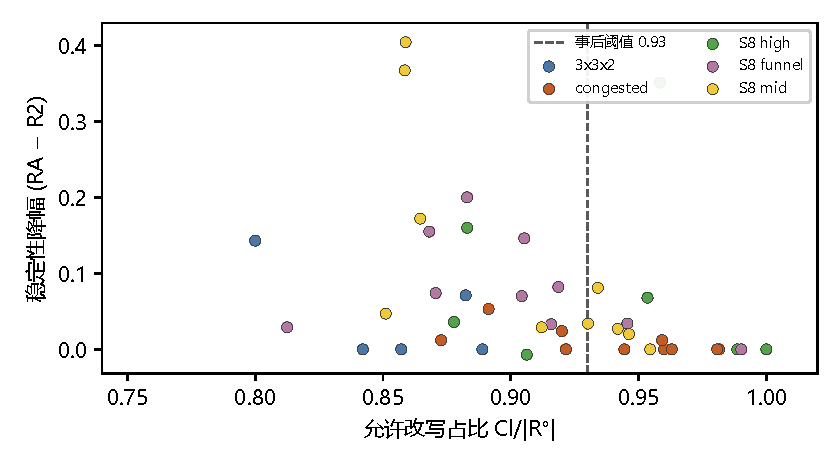
\includegraphics[width=0.92\linewidth]{figures/fig_strc_worth_CN}
\caption{E7 事后规则：允许改写占比与稳定性降幅（\(\NPairs\) 对，R2 对 RA）。
虚线为样本内阈值 \(\WorthThresh\)；纵轴为正表示按影响集划界后改动比例更低。}
\Description{散点图，横轴为预约影响集占尚未结束占用的比例，纵轴为不按影响集划界相对划界多改的占用比例，
五个算例用不同颜色区分，一条竖虚线标在 \WorthThresh。点大致从左上到右下。}
\label{fig:worth}
\end{figure}

综合四种方法的结果：在「不改写已经结束的占用」且「响应须在毫秒量级」两个约束下，
\textbf{按影响集划界的净收益只体现在改写量上。}
\textbf{在速度与完工时间相同的条件下，不划界需多改写约 \(6\) 个百分点的占用（相对增加约 \(12\%\)）}，
而划界\emph{不}带来速度或完工时间上的优势。
放宽耗时约束后，更短的完工时间仍来自热启动搜索（第~\ref{sec:e5}~节），
但其耗时已超出毫秒量级。

\subsection{扰动规模扫描}
\label{sec:scale}

表~\ref{tab:scale} 与图~\ref{fig:scale} 报告 \(\varphi\) 扫描
（\texttt{congested\_8x4x4}, \(\NSeeds\) 个随机种子；R0+ 预算 \(2\)\,s）。
逐档结果见表；\(C_{\max}\) 仍全由 R0+ 更优，与第~\ref{sec:e5}~节一致。
小例 \texttt{example\_3x3x2} 上同样每格可行（\(\NSeeds\) 个随机种子 \(\times\) 五个
\(\varphi\) 值），有界修复约 \(1\)\,ms 量级，
耗时比 \(\SpeedLo\times\)--\(\SpeedHi\times\)（跨两个算例的逐格极值）。该比值以 R0+ 的\emph{预算}为分子、有界修复的实测挂钟为分母，而 R0+ 在 \(C_{\max}\) 上更优，
故不应理解为同等质量下的加速比。

本节的有界修复启用了失败后扩大范围，故结果与 E3、E5 不可直接比较。
即使扰动比例升至 \(\varphi=1\)（全部未来工序受扰动），算法耗时仍在十毫秒量级，不随扰动规模显著增长；
这一耗时来自单遍改路（第~\ref{sec:cheap}~节）。

\begin{table}[t]
\centering
\caption{扰动规模对照（\texttt{congested\_8x4x4}, \(\NSeeds\) 个随机种子平均）。
有界修复含扩大范围；R0+ 预算 \(2\)\,s。离散度按四分位距报告：STRC 耗时全扫描极差为
\ScaleMsMin--\ScaleMsMax\,ms,R0+ \(C_{\max}\) 的逐档 IQR 在 \ScaleCmaxIqrLo--\ScaleCmaxIqrHi
之间。\textbf{「耗时比」一列在最小两档上的档内 IQR 已超过该列的档间起落，
故它只反映量级，不指示随 \(\varphi\) 变化的趋势。}该列为\emph{逐格}比值的档均值（先配对、后统计），
因此不等于相邻两列档均值之比；由 \(1/x\) 的凸性，两者一般不同，复算时应使用逐格数据。
分子是 R0+ 的挂钟\emph{预算}而非其实测耗时，故这不是同质量下的比较（第~\ref{sec:protocol}~节）。}
\label{tab:scale}
\small
\begin{tabular}{@{}rcccc@{}}
\toprule
\(\varphi\) & STRC 可行 & STRC\,ms & R0+ \(C_{\max}\) & 耗时比 \\
\midrule
\(0.10\) & \(100\%\) & \(9.1\)  & \(103.5\) & \(406\times\) \\
\(0.25\) & \(100\%\) & \(11.1\) & \(107.0\) & \(325\times\) \\
\(0.50\) & \(100\%\) & \(8.6\)  & \(111.8\) & \(333\times\) \\
\(0.75\) & \(100\%\) & \(8.4\)  & \(125.8\) & \(254\times\) \\
\(1.00\) & \(100\%\) & \(10.7\) & \(148.1\) & \(203\times\) \\
\bottomrule
\end{tabular}
\end{table}

\begin{figure}[t]
\centering
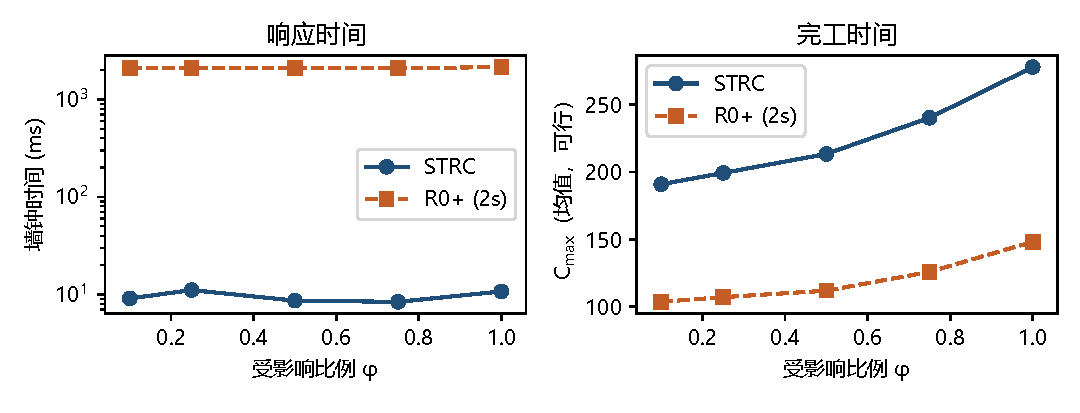
\includegraphics[width=\linewidth]{figures/fig_strc_scale_CN}
\caption{扰动规模扫描（\texttt{congested\_8x4x4}, \(\NSeeds\) 个随机种子）：
有界修复与 R0+ 的算法耗时（对数轴）与完工时间随 \(\varphi\) 变化。曲线取逐档均值，
离散度口径与表~\ref{tab:scale} 同（四分位距）；耗时一侧全扫描极差
\ScaleMsMin--\ScaleMsMax\,ms，始终在十毫秒量级，这是本节结论所依据的唯一结果。}
\Description{两条随扰动比例变化的曲线。算法耗时画在对数纵轴上：有界修复始终在
十毫秒量级、不随比例上升而显著增长，全局重调度固定在两秒的预算线上。完工时间一侧，
全局重调度随扰动比例增大而缓慢上升，但始终低于有界修复。}
\label{fig:scale}
\end{figure}

\subsection{E8：算例规模上的外推}
\label{sec:instscale}

上一节扫描的是\emph{扰动}的规模，算例始终为 \(8\) 工件 \(4\) 机。本节转向另一维：固定扰动协议，
扩大算例本身。此处的关键不在耗时（耗时不显著增长是可以预期的），而在于\textbf{影响集占比是否会
随规模增大而接近 \(1\)，使「有界」失去实际意义}。

规模序列取工件数 \(2k\)、机器数 \(k\)、车辆数 \(k\),\(k=4,\dots,10\)，即 \(8\times4\times4\) 到
\(\ScaleJobsHi\times\ScaleMachHi\times\ScaleMachHi\)，共 \(\ScaleKs\) 档 \(\times\)
\(\NSeeds\) 个随机种子 \(=\ScalePairs\) 对。拥堵档、异构度、柔性度、运输/加工时长比与装卸站
最小割、远端割全部按同一目标标定，\emph{只改变规模}。三个对照方法与第~\ref{sec:cheap}~节定义相同。

\begin{table}[t]
\centering
\caption{E8 算例规模扫描（\(\ScaleKs\) 档 \(\times\) \(\NSeeds\) 个随机种子）。
「影响集」为预约影响集占\emph{全表}之比，该比的可达上界是 \(|R^{\circ}|/|R|\)、本批均值约
\ScaleAliveShare；换以可改写集合为分母则为 \ScaleCloAliveLo--\ScaleCloAliveHi（见正文）。
耗时取中位数，「RD/R2」一列即两列\emph{中位数之比}；正文讨论其单调性时用的是逐格配对后的
档均值，两种口径的档间起落一致但数值不同。末列为 R2 对 RS 的 \(C_{\max}\) 胜负。}
\label{tab:instscale}
\small
\begin{tabular}{@{}lrccccc@{}}
\toprule
规模 & \(|R|\) & 影响集 & R2\,ms & RD\,ms & RD/R2 & R2 对 RS \\
\midrule
\(8\times4\times4\)    & \(148\) & \(0.561\) & \(2.9\)  & \(4.4\)  & \(1.5\times\) & \(7/1/2\) \\
\(10\times5\times5\)   & \(172\) & \(0.485\) & \(3.2\)  & \(6.1\)  & \(1.9\times\) & \(9/0/1\) \\
\(12\times6\times6\)   & \(230\) & \(0.481\) & \(4.5\)  & \(10.7\) & \(2.4\times\) & \(7/1/2\) \\
\(14\times7\times7\)   & \(281\) & \(0.492\) & \(6.1\)  & \(14.5\) & \(2.4\times\) & \(8/0/2\) \\
\(16\times8\times8\)   & \(291\) & \(0.534\) & \(6.4\)  & \(16.4\) & \(2.6\times\) & \(10/0/0\) \\
\(18\times9\times9\)   & \(356\) & \(0.535\) & \(8.2\)  & \(26.4\) & \(3.2\times\) & \(10/0/0\) \\
\(20\times10\times10\) & \(402\) & \(0.476\) & \(10.4\) & \(34.2\) & \(3.3\times\) & \(10/0/0\) \\
\bottomrule
\end{tabular}
\end{table}

逐档结果见表~\ref{tab:instscale}。

\textbf{影响集占比不随规模增大而上升，但「是否接近 \(1\)」须换用恰当的分母才能回答。}
七档 \(\mathrm{Cl}/|R|\) 在 \ScaleCloLo--\ScaleCloHi 之间波动，且不单调
（首档最高、末档最低，第五、六两档回到 \(0.53\) 以上）。由于 \(\mathrm{Cl}\) 只包含
\(t_{\mathrm{now}}\) 之后尚未结束的占用，而本批 \(|R^{\circ}|/|R|\) 均值仅为 \ScaleAliveShare，
\(\mathrm{Cl}/|R|\) 的可达上界约为 \ScaleAliveShare 而非 \(1\)。以可改写集合为分母时，
七档 \(\mathrm{Cl}/|R^{\circ}|\) 落在 \ScaleCloAliveLo--\ScaleCloAliveHi（逐格最高为 \(1.00\)），
与第~\ref{sec:e6}、\ref{sec:cheap}~两节主批次的 \ClosureAliveFrac\ 同量级。
因此本节表明\emph{占比不随规模增大而上升}，但影响集相对可改写集合并不小（注~\ref{rem:minimality}）；
七档数据也不足以支持渐近结论。

\textbf{算法耗时的增长快于占用总数的增长。} \(|R|\) 增至 \(2.7\) 倍时，R2 的耗时中位数从
\(2.9\)\,ms 增至 \ScaleMsHi\,ms，即 \(3.6\) 倍，仍在十毫秒量级；七档数据不足以确定增长阶。第 1 级改路的可行格数为 \ScaleFeasFirst；
唯一失败的一格（\(10\times5\times5\)，随机种子 \(42\)）经失败后扩大范围在第 \(3\) 轮恢复可行，
总耗时 \(12.0\)\,ms，完工时间与第 1 级尝试相同，故最终可行格数为 \ScaleFeasAll。

\textbf{两种对照方法的耗时差距随规模增大。} 耗时最短的全局重算与有界修复的耗时比
从 \ScaleRatioLo\(\times\) 升至 \ScaleRatioHi\(\times\)，即规模越大，全局重算的耗时代价越高。
逐档比值\emph{并不单调}（逐格配对后的档均值在 \(k=6\to 7\) 处回落），但两端相差 \(1.8\)，
远大于任一档内不超过 \(0.74\) 的四分位距，故\emph{总体上升}并非噪声。

与不按影响集划界的全局右移相比，R2 的 \(C_{\max}\) 胜负在最后三档均为 \(10/0/0\)，前四档则在
\(7\)--\(9\) 胜之间，无单调变化；每档只有 \NSeeds\ 格，不足以判断趋势。

\textbf{口径限制。} 这一规模序列只有一个拥堵档和一个算例随机种子（每档的算例均由随机种子
\(42\) 生成），只检验\emph{规模}这一维；第~\ref{sec:e6}、\ref{sec:scale}~两节的扫描未在这批算例上重新运行。
就贡献而言，本节为 C2 的有界性补充了规模方向的证据：占比在这七档上没有上升。

\subsection{外部布局批次的复现}
\label{sec:pubrepro}

第~\ref{sec:protocol}~节第二批把布局出处换成外部来源后，\(\NPubPairs\) 个算例--随机种子对上
E1、E2、E3、E5 的结果与主批次\emph{逐项同向}：
工序依赖图给出空范围 \PubPassMiss，结构包含性（即泄漏计 \(0\)）\PubPassClosed，
集外字段逐条不变 \PubPassInvar；边界消融下第 1 级改路的可行格数为 \PubFeasRone，
按预约影响集划界为 \PubFeasRtwo。E1 协议下影响集占比的逐布局中位数落在
\PubEoneFracLo--\PubEoneFracHi；同口径的主批次结果是 \NPairs\ 对合并后的中位数 \EoneFracMed
（\EoneCloLo--\EoneCloHi\ 是逐算例\emph{均值}的极差，口径不同）。
外部批次整体略低，但两者均约为一半，且偏低幅度与算例间差异同量级（第~\ref{sec:e1}~节图注）。
与全局重调度的权衡亦无变化：\PubEfiveNoCross\ 个预算点上 R0+ 的 \(C_{\max}\) 更优，
余下 \(1\) 点两法持平（\texttt{LyuL6\_8m}，随机种子 \(2024\)，预算 \(0.2\)\,s），无一点更差。
这批与主批次使用同一份 E5 代码和同一组参数，故第~\ref{sec:e5}~节按 \(\EfiveCells\) 个
算例--随机种子格合并分析两批；持平的一格同样满足该节的单调性判断，交叉点仍不存在。

这一批用于检验上述现象是否只在本文设计的布局上成立：结果在一批并非由本文选定的拓扑上同样成立，
故 C1 与 C2 的对象层不依赖本文的布局设计。这批算例唯一改变的是结构可预测性的结论（第~\ref{sec:e4}~节）。

\subsection{小结}
\label{sec:exp_summary}

本章结果按其支撑的贡献层归并；各项局限及其影响的层次集中见第~\ref{sec:limitations}~节。

\textbf{对象层}（C1、C2：按什么对象划界、划出的集合是否唯一确定）由四组结果支撑。
走廊阻断下工序依赖图上的范围为空，而原排程确已不可行（E1,\(\NPairs\) 对上 \(\PassMiss\)）；
预约影响集对依赖边封闭，集外字段逐条不变(E2,\(\PassClosed\)、\(\PassInvar\))；
同一套改路程序只更换划界对象，恢复可行率即由 \(\FeasRone\) 变为 \(\FeasRtwo\)(E3)，
因此可行与否取决于划界对象，而非改路程序的优劣；在四类扰动与两种划界对象的交叉中 A/B 二分无例外，
且 A 类上预约影响集均包含工序依赖图划界的结果(E6)。
命题~\ref{prop:miss}--\ref{prop:outside} 给出对应的结构陈述，
其中命题~\ref{prop:outside} 仍只作充分条件。

\textbf{净收益层}（C3：这样划界带来什么收益）只由一组结果支撑：换用不按影响集限制范围的对照
（RA，与 R2 使用同一套改路，同样不改写已经结束的占用）后，算法耗时与 \(C_{\max}\) 几乎不变，
改动比例却由 \ResFracCheapRtwo\ 升至 \ResFracAllFuture（逐格 \RAStabWTL,\(p=\RAStabP\)；
第~\ref{sec:cheap}~节）。故毫秒量级的响应来自单遍改路而非影响集，
\textbf{改写量的减少只能由这一对照得出}。与热启动全局重调度相比，有界修复在 \(C_{\max}\) 上
无一格更优，放宽预算也不出现反超(E5);E7 则排除了「对照方法耗时过长」这一解释。

其余结果为限定性结果：算例规模已扩展至 \(\ScaleJobsHi\) 工件
\(\ScaleMachHi\) 机，以可改写集合为分母的影响集占比未随规模上升(E8)；
结构可预测性是负结果(E4)。第二批算例（\(\NPubPairs\) 对）只检验上述现象是否依赖
本文自行设计的布局，E1、E2、E3、E5 的结果逐项复现。

%% =====================================================================
\section{总结}
\label{sec:conclusion}
%% =====================================================================

本文有三项贡献。\textbf{其一}(C1)，指出了一类工序依赖图无法刻画的失效：走廊阻断不改变任何工序指派，
按受影响工序划出的范围为空，而原排程确已不可行（\(\NPairs\) 对上 \(\PassMiss\)，第~\ref{sec:e1}~节）。
\textbf{其二}(C2)，以 \STRC 得到的预约影响集作为重调度范围：依赖关系一经给定，一条占用是否属于该集合即
唯一确定，集内没有指向集外的依赖边（\(\PassClosed\)、\(\PassInvar\)，第~\ref{sec:e2}~节）。
\textbf{其三}(C3)，给出与该划界相匹配的局部恢复，并区分各项结果的来源：同一套改路程序只更换划界对象，
恢复可行率即由 \(\FeasRone\) 变为 \(\FeasRtwo\)（第~\ref{sec:e3}~节），
因此可行与否取决于划界对象，而非改路程序的优劣。

让行关系、集内改路而集外保持原计划、失败后扩大允许改写的范围均沿用既有文献
（第~\ref{sec:rw_claim}~节）。本文的主张是：
工序依赖图按定义不含走廊占用之间的让行关系，因而无法刻画只使占用失效的扰动；
在预约依赖图上划界后，须改写的占用由既定先后关系唯一确定，而非取决于启发式半径。

将允许改写的集合从预约影响集换为「\(t_{\mathrm{now}}\) 之后尚未结束的全部占用」、
其余条件不变时，算法耗时与完工时间几乎不变，改动比例却由 \ResFracCheapRtwo\ 升至
\ResFracAllFuture（第~\ref{sec:cheap}~节）。
故毫秒量级的响应来自单遍改路、不重新启动搜索；\textbf{改写量的减少只能由这一对照得出，
它体现的是命题~\ref{prop:outside} 所保证的性质：集外占用保持原计划}。
收益幅度取决于影响集比该平凡上界小多少，两者接近时收益趋于消失。

\subsection{局限}
\label{sec:limitations}

以下四条按对前文结果的影响排序，第~\ref{sec:future}~节逐条给出推进方向。

\begin{enumerate}[leftmargin=1.6em,itemsep=0.35em]
\item \textbf{完工时间劣于不改写已结束占用的热启动全局重调度，且放宽预算不出现反超。}
有界修复以完工时间换取算法耗时，而这一劣势在所测的 \(\EfiveCells\) 个算例--随机种子格上
不随预算放宽而反转（第~\ref{sec:e5}~节）。
该局限关系到划界的净收益，而不涉及对象层的结论；改写量的比较见第~\ref{sec:cheap}~节。

\item \textbf{对预约影响集，命题~\ref{prop:outside} 的保证只是充分条件，依赖边集未经独立的
穷尽检验，允许改写的集合不紧，其规模也不能由仅依赖路网的静态指标预测。}
影响集覆盖 \(t_{\mathrm{now}}\) 之后尚未结束占用的约 \(\ClosureAliveFrac\)（注~\ref{rem:minimality}），
净收益的幅度取决于影响集小于该平凡上界的程度，两者接近时收益趋于消失。
静态割这一族指标已由第~\ref{sec:e4}~节排除，路网几何与影响集规模的一般关系仍待研究。
该局限关系到对象层保证的强度与紧度，不影响「按工序依赖图划界会给出空范围」这一诊断。

\item \textbf{实现覆盖小于正文所述的问题范围：B 类扰动仅以改路响应，A 类另允许换车与改派
但不改变加工顺序，且由假设 A3 只做一次响应。}
放开加工顺序即向全局重调度退化，「有界」随之失去意义；扰动流、预测误差与滚动响应均未涉及。
规模一维已扩展至 \(\ScaleJobsHi\) 工件 \(\ScaleMachHi\) 机且影响集占比未随规模上升，
但所扫档数不足以支撑渐近论断。该局限限制了结果向更大规模与连续扰动的外推。

\item \textbf{外部参照缺位：这一类研究没有可换用的公开基准，算例出处只外部化到拓扑一层，
结果亦未在第二套实现上复现。}
公开算例族~\cite{homayouni2021production,bilge1995time} 把运输时间发布为机器间行程时间矩阵而不是路网，两族共 \(11\) 张布局逐张检验没有一张
能还原成与所发布矩阵一致的无向走廊图，\(R\)、\(G_R\)、\(\mathrm{Cl}(\cdot)\) 与 B 类扰动
在其上均无法定义（第~\ref{sec:protocol}~节）。
第二批算例按 Lyu 等~\cite{lyu2019approach} 的附录布局构造，布局因此不再由本文设计，
但逐段行驶时间与工件数据仍出自本文，故不能用来复现 Lyu 或 van Os~\cite{vanos2026exact} 的参照值，
其覆盖范围也小于主批次。该局限关系到外部效度，同一实现内各对照之间的相对结果不受影响。
\end{enumerate}

\subsection{后续工作}
\label{sec:future}

下列四条与上一节的四个局限一一对应。

\textbf{一、缩小完工时间上的差距}（局限 \(1\)）。
在主批次中，前缀解码不改写已结束的占用（E5 的 \(18\) 个预算点越界数为 \(\RzeroPastLo\),
E7 上 RD 为 \RedecodeBad），故局限 1 仅涉及 \(C_{\max}\) 本身。
若要缩小差距，须在不改写已结束占用的前提下进行有限度的改派或改序，但这会使方法向全局重调度退化。

\textbf{二、使预约影响集的保证更完备、更紧，并刻画其规模}（局限 \(2\)）。
\emph{完备性}：在当前让行边集下，试探泄漏为 \ProbeLeaks；
下一步是采用其他扰动形态（例如缩短占用，或延后超过 \(1\) 个时间单位）进行试探，而非继续补充同类依赖边。
\emph{紧度}指向最小允许改写集合：在固定修复能力下定义最小性，
并给出影响集与之的差距，这是把「有界」从充分条件推进到紧界的必要步骤；当前影响集覆盖约
\(\ClosureAliveFrac\) 的尚未结束占用，两者的差距可能相当大。\emph{规模刻画}目前只有一条
事后规则（允许改写占比，图~\ref{fig:worth}），但它随排程而变，须改用可在扰动前计算的指标。
第~\ref{sec:e4}~节已排除静态割这一族指标：它在实际布局上取值恒定，而同一张路网上
仅改变机器配置，影响集占比即发生变化，\(4\times 4\) 路网上由 \(4\) 机改为 \(5\) 机即变化 \PubCloSpread,
\(5\times 5\) 路网上改变三种配置（\(6\)、\(7\)、\(8\) 机）变化 \PubCloSpreadBig。
这提示起作用的可能是\emph{需求的空间分布}，而非路网所提供的通行能力。
下一个候选是 \(t_{\mathrm{now}}\) 邻域内的走廊占用时序密度，例如受扰走廊在其繁忙窗口内的
重叠占用条数、以及该走廊在让行图上的出度。这类量随排程而变，不再是纯拓扑量，
「可预测性」的提法也须随之改为给定布局\emph{与当前排程}预测规模。

\textbf{三、放开假设 A3}（局限 \(3\);A3 为单次、完全观测）。
下一步不在于进一步开放改序，而在于放开该假设，考察影响集在连续扰动下是否会累积膨胀，
以及两次修复之间是否需要显式的「归位」步骤。

\textbf{四、使时间标定同样采用外部来源}（局限 \(4\)）。布局已采用外部来源；时间标定方面，
仍需一份同时发布\emph{排他路网与逐段时长}的算例族，自建边权扫描不能替代。
第二套独立实现无须单独开展，可在复现上述任一项时一并完成。

%% 规范项收口:基金、致谢、利益冲突三项按期刊通例齐备。
%% acmart 的 acks 环境在 review/anonymous 模式下自动隐去,故匿名投稿无需手工删。
\begin{acks}
本文工作由 <待填：基金项目名称与编号> 资助。
作者感谢匿名审稿人对实验口径与结论边界提出的意见。
\end{acks}

\section*{利益冲突声明}
作者声明不存在与本文工作相关的利益冲突。

\bibliographystyle{ACM-Reference-Format}
\bibliography{reference-base}

\end{document}
